\documentclass[
    Department = {{Dipartimento di Matematica Informatica e Geoscienze}},
    DepartmentCode = mige,
    Course = {{Corso di Laurea in Intelligenza Artificiale e Data Analytics}},
    Title = {{Judo: Verso un Tatami più Sicuro}},
    Subtitle = {{Dinamica e Controllo per lo studio degli infortuni a mezzo di un nuovo modello matematico}},
    Student = {{Ludovico Urbani}},
    StudentID = SM3201372,
    Teacher = {{Prof.~Alberto d'Onofrio}}
]{unitsthesis}

\addbibresource{main.bib}
\setcounter{biburllcpenalty}{7000}
\setcounter{biburlucpenalty}{8000}

\makeatletter
\addto\extrasitalian{%
    \renewcommand{\sectionautorefname}{Sezione}%
    \renewcommand{\subsectionautorefname}{Sezione}%
    \renewcommand{\subsubsectionautorefname}{Sezione}%
    \renewcommand{\figureautorefname}{Figura}%
    \renewcommand{\tableautorefname}{Tabella}%
}
\makeatother

\usepackage{tikz}
\usetikzlibrary{arrows.meta, calc, positioning, decorations.pathreplacing}

\definecolor{ColorS}{HTML}{009933}
\definecolor{ColorP}{HTML}{336699}
\definecolor{ColorI}{HTML}{EE0000}
\definecolor{ColorM}{HTML}{FFAD00}

\setcounter{tocdepth}{1}

% Figures and tables never float past the end of their subsection
\usepackage[section]{placeins}
\NewCommandCopy{\placeinsSubsection}{\subsection}
\RenewDocumentCommand{\subsection}{}{\FloatBarrier\placeinsSubsection}
\NewCommandCopy{\placeinsSubsubsection}{\subsubsection}
\RenewDocumentCommand{\subsubsection}{}{\FloatBarrier\placeinsSubsubsection}

\graphicspath{ {./images} }

\captionsetup{justification = centering}
\NewDocumentCommand{\creditcaption}{O{#2} m m}{%
    \caption[#1]{#2\\{\footnotesize\itshape #3}}%
}

\SetTblrInner{
    hline{1,Z} = {0.08em},
    hline{2} = {0.05em}
}

\begin{document}
    \chapter{Introduzione}

\section{Il judo e la sua storia}

Il judo nasce in Giappone alla fine dell'Ottocento per opera di Jigoro Kano, che nel 1882 fonda a Tokyo il Kodokan, il dojo da cui il judo si è diffuso in tutto il mondo~\cite{kano1986}. Kano aveva studiato per anni il jujutsu, cioè l'insieme delle tecniche di difesa a mani nude dei samurai, e ne aveva colto sia l'efficacia sia i limiti: molte tecniche erano pericolose e non potevano essere praticate liberamente senza rischiare gravi infortuni. Da questa esperienza nasce l'idea di un metodo educativo nuovo, che conservasse i principi tecnici, eliminasse le tecniche troppo pericolose e permettesse di allenarsi con un compagno per raggiungere una mutua crescita. \par

Il nome stesso riassume questa idea, infatti la parola judo significa ``via dell'adattabilità'' o ``via della flessibilità''. Invece di opporsi con la forza alla forza dell'avversario, il judoka cerca di sfruttarla, sbilanciandolo e usando il suo stesso movimento per proiettarlo o controllarlo a terra. Kano riassume il judo in due principi: \textit{Seiryoku-zenyo}, il miglior impiego dell'energia, e \textit{Jita-kyoei}, il principio della mutua crescita, secondo cui lo sviluppo del singolo passa attraverso la collaborazione con gli altri~\cite{kano1986}. Il judo nasce quindi non soltanto come arte di combattimento, ma come metodo di educazione fisica e morale. \par

\begin{figure}[ht]
    \centering
    \includegraphics[width = 0.5\textwidth]{pictures/kano.jpg}
    \creditcaption[Statua di Jigoro Kano]{Statua di Jigoro Kano, di F. Asakura, davanti al Kodokan di Tokyo.}{Foto di H. Probell, Wikimedia Commons, licenza CC BY-SA 2.5, \url{https://commons.wikimedia.org/wiki/File:Kodokan_Jigoro_Kano_Statue.jpg}}
\end{figure}

Per rendere possibili le proiezioni in sicurezza, il judo dà grande importanza alle tecniche di caduta (ukemi), che ogni praticante impara fin dalle prime lezioni e che permettono di essere proiettati senza farsi male. L'allenamento si svolge sempre in coppia sul tatami (un tappeto progettato apposta per attutire meglio le cadute) e alterna diversi tipi di esercizio: la preparazione fisica, lo studio delle tecniche, la loro ripetizione con un compagno e il combattimento libero in piedi e a terra (randori). Proprio il randori, in cui due atleti combattono liberamente cercando di applicare le proprie tecniche, è il cuore dell'allenamento e allo stesso tempo il momento in cui il corpo è sottoposto al maggior rischio di infortunio.

\section{Dal judo educativo al judo sportivo}

Nel corso del Novecento il judo si diffonde rapidamente fuori dal Giappone e assume sempre più il carattere di sport. Nel 1951 nasce la Federazione Internazionale di Judo, che unifica i regolamenti e organizza le competizioni internazionali, e nel 1964, ai Giochi Olimpici di Tokyo, il judo maschile entra per la prima volta nel programma olimpico. Dal 1992, con i Giochi di Barcellona, anche il judo femminile fa parte del programma olimpico~\cite{ijfhistory}. \par

L'ingresso del judo nel panorama olimpico ha trasformato profondamente questa disciplina. Le competizioni sono state suddivise in categorie di peso, i regolamenti sono stati più volte rivisti con l'obiettivo di rendere gli incontri più dinamici e spettacolari, e il numero di gare a livello internazionale è aumentato. Per un atleta di alto livello, il judo è diventato una disciplina che richiede, oltre alla tecnica, una preparazione fisica molto sviluppata. Gli studi sul profilo fisiologico degli atleti d'élite evidenziano che il judo richiede soprattutto un'elevata potenza anaerobica, in particolare della parte superiore del corpo, una buona capacità aerobica e una bassa percentuale di massa grassa, con l'eccezione delle categorie più pesanti~\cite{franchini2011}. \par

\begin{figure}[ht]
    \centering
    \includegraphics[width = 0.8\textwidth]{pictures/throw.jpg}
    \creditcaption[Proiezione di judo]{Finale pesi massimi, Parigi 2024.}{Foto \textcopyright~International Judo Federation, \url{https://www.ijf.org/competition/2653/photos?id_weight=7}}
\end{figure}

Di conseguenza, anche l'allenamento ha subito cambiamenti. Un atleta di alto livello si allena spesso più volte al giorno, alternando sedute tecniche, sedute di randori ad alta intensità e sedute di preparazione fisica, e affronta periodi di preparazione intensa in vista delle gare più importanti. Nei raduni e nei centri di allenamento nazionali capita spesso di trovare molti atleti sullo stesso tatami, che si allenano a coppie cambiando frequentemente compagno. A queste esigenze si aggiunge, per molti atleti, la necessità di rientrare nella propria categoria di peso, che comporta talvolta perdite di peso rapide nei giorni che precedono la gara. \par

Questa evoluzione ha portato a prestazioni sempre più elevate, ma ha anche aumentato le sollecitazioni a cui è sottoposto il corpo degli atleti. Un carico di allenamento elevato e mal distribuito, unito a un recupero insufficiente, è oggi considerato uno dei principali fattori di rischio di infortunio nello sport~\cite{soligard2016}. Non è però il carico in sé a essere dannoso, infatti un carico elevato, raggiunto in modo graduale, rende gli atleti più resistenti, mentre sono gli aumenti bruschi e non accompagnati da un adeguato recupero a far crescere il rischio~\cite{gabbett2016}.

\section{Gli infortuni nel judo}

Il judo è uno sport di combattimento e di contatto, nel quale gli atleti vengono continuamente proiettati, cadono, si oppongono con forza alle tecniche dell'avversario e lottano per ottenere il controllo a terra. Non sorprende quindi che gli infortuni siano frequenti. Una revisione sistematica degli studi sugli infortuni nel judo indica che i più comuni sono le distorsioni, gli stiramenti e le contusioni, che interessano soprattutto il ginocchio, la spalla e le dita, e che il meccanismo più frequente è l'essere proiettati. Gli infortuni gravi, come quelli alla testa e alla colonna vertebrale, sono rari, mentre tra i problemi cronici si riscontrano soprattutto quelli alle articolazioni delle dita, alla parte bassa della schiena, alle anche e alle ginocchia~\cite{pocecco2013}. \par

\begin{figure}[ht]
    \centering
    \includegraphics[width = 0.8\textwidth]{pictures/training-camp.jpg}
    \creditcaption[Tatami durante una sessione di allenamento]{Tatami durante una sessione di allenamento, Judo Training Camp, Roma 2026.}{Foto \textcopyright~FIJLKAM, \url{https://www.fijlkam.it/media-fijlkam/galleria-fotografica/galleria-fotografica/2026/judo-training-camp-roma-2026.html}}
\end{figure}

Ad alto livello il judo risulta tra gli sport di combattimento più rischiosi. Un'analisi degli infortuni negli sport di combattimento in tre Olimpiadi consecutive, Pechino 2008, Londra 2012 e Rio de Janeiro 2016, ha mostrato che il judo ha il tasso di infortuni più alto tra gli sport considerati, con circa $9.6$ infortuni ogni $1000$ minuti di gara. Inoltre, più di un terzo degli infortuni nel judo, il $35.9\%$, ha costretto l'atleta a fermarsi per più di una settimana~\cite{lystad2021}. \par

Gli infortuni, però, non si verificano soltanto in gara. La maggior parte del tempo di un atleta è dedicata all'allenamento, ed è proprio lì che si accumulano la fatica e le sollecitazioni ripetute. Uno studio prospettico condotto per quattro anni nel centro di allenamento della nazionale coreana di judo ha registrato $782$ infortuni, pari a circa quattro infortuni per atleta ogni anno. Circa la metà erano lievi, con meno di quattro giorni di cure, e la zona più colpita era la parte inferiore del corpo, con il $44.2\%$ degli infortuni, seguita dalla parte superiore, con il $29.8\%$, e dal tronco, con il $20.3\%$~\cite{kim2015}. \par

Oltre al carico di allenamento, la letteratura indica altri fattori che possono aumentare il rischio. Uno di questi è la perdita di peso prima delle gare: uno studio sugli infortuni durante le competizioni ha osservato che gli atleti che avevano perso peso prima della gara si infortunavano più spesso, e gli autori sconsigliano questa pratica~\cite{green2007}. Altri fattori discussi sono l'alimentazione, l'idratazione e gli aspetti psicologici~\cite{pocecco2013}. \par

Le conseguenze di un infortunio vanno oltre il dolore e le cure. Un atleta infortunato deve interrompere o ridurre l'allenamento, perde parte della preparazione e, se torna ad allenarsi prima di essere completamente guarito, può essere più esposto a nuovi infortuni. Per una squadra o una palestra, inoltre, gli infortuni riducono il numero di atleti disponibili e possono portare alcuni di loro ad abbandonare l'attività.

\section{Perché un modello matematico}

Gli studi citati descrivono con precisione quanti infortuni avvengono, di che tipo sono e in quali parti del corpo si localizzano. Ciò che risulta più difficile da studiare è invece il modo in cui gli infortuni si sviluppano nel tempo all'interno di un gruppo che si allena insieme. In una palestra o in un raduno, infatti, gli infortuni non sono eventi isolati: la fatica si accumula seduta dopo seduta e aumenta il rischio per tutti gli atleti; un tatami affollato rende più probabili gli scontri tra coppie; un atleta che ha subito un infortunio lieve continua spesso ad allenarsi in condizioni non ottimali ed è quindi più esposto a un nuovo infortunio; e gli atleti che si infortunano sono anche quelli che più facilmente abbandonano il gruppo. \par

Questi fenomeni sono legati tra loro, e il loro effetto complessivo non è facile da prevedere in modo intuitivo. Ridurre il carico di una seduta, ad esempio, diminuisce la fatica e quindi gli infortuni, ma riduce anche il beneficio dell'allenamento; aumentare la prevenzione riduce gli infortuni, ma richiede tempo e attenzione; e una riduzione degli infortuni ha a sua volta effetti sulla composizione del gruppo e sugli abbandoni. Studiare queste interazioni direttamente sugli atleti sarebbe difficile e, in molti casi, non accettabile: non è possibile sottoporre un gruppo a un carico eccessivo solo per osservare quanti infortuni produce. \par

Un modello matematico permette invece di studiare queste interazioni in modo controllato. Descrivendo con delle equazioni come cambia il gruppo da una seduta all'altra, è possibile simulare periodi di allenamento diversi, confrontare scenari differenti e valutare l'effetto di una strategia di prevenzione prima di applicarla. Il modello, naturalmente, è una semplificazione della realtà, e i suoi risultati vanno interpretati con cautela: non sostituisce l'esperienza dell'allenatore né i dati raccolti sul campo, ma offre uno strumento per ragionare in modo quantitativo su fenomeni che altrimenti si possono valutare solo a intuito. \par

In questa tesi proponiamo un modello di questo tipo. Il modello divide gli atleti di un gruppo in quattro popolazioni, cioè i sani, gli atleti con infortuni pregressi, gli infortunati e gli atleti che si allenano nonostante un infortunio lieve, e descrive come gli atleti passano da una popolazione all'altra in funzione della fatica accumulata, della densità di atleti sul tatami e dei flussi di ingresso e di abbandono del gruppo. Al modello viene poi aggiunto un controllo, che rappresenta la prevenzione messa in atto dall'allenatore, per studiare quanto e come la prevenzione possa ridurre gli infortuni.
    \chapter{Introduzione del modello}

Introduciamo un modello matematico a tempo discreto con l'obiettivo di rappresentare in modo sintetico come la composizione del gruppo e lo stato di affaticamento medio varino nel tempo in risposta al carico di allenamento, agli infortuni e ai flussi di ingresso e uscita dalla popolazione. Il modello non ha la pretesa di descrivere il comportamento individuale di ogni atleta, ma di catturare le tendenze aggregate di un gruppo sufficientemente numeroso, per il quale le dinamiche collettive sono più rilevanti delle fluttuazioni individuali. In altre parole, il modello si colloca a un livello di astrazione intermedio: è sufficientemente dettagliato da distinguere stati diversi degli atleti e da descrivere l'evoluzione della fatica, ma sufficientemente aggregato da rimanere trattabile analiticamente e da non richiedere la simulazione di ogni singolo individuo. \par

La struttura del modello, che divide gli atleti in popolazioni e descrive i passaggi da una popolazione all'altra, si ispira ai modelli a compartimenti dell'epidemiologia matematica, introdotti da Kermack e McKendrick per lo studio delle epidemie e oggi ampiamente diffusi~\cite{kermack1927}. Come avviene per molti di questi modelli, la dinamica è descritta da un sistema di equazioni alle differenze, cioè a tempo discreto~\cite{brauer2010}. \par

Il modello è formulato a tempo discreto, con $t = 0, 1, \dots, T$, dove $T$ è l'orizzonte temporale considerato. Si assume che le sedute di allenamento siano distribuite circa omogeneamente nel tempo, così che ogni passo $t \to t+1$ corrisponda a una seduta e il tempo che intercorre tra due sedute sia approssimativamente lo stesso. \\
Se consideriamo ad esempio un programma di allenamento basato su una seduta al giorno, possiamo dire che ogni passo $t$ corrisponda a un giorno. In questo modo è possibile confrontare anche il recupero tra due sedute consecutive, perché l'intervallo di tempo tra un passo e il successivo è pressoché costante per ipotesi. \par

Questa scelta è motivata dal fatto che gli allenamenti sono eventi discreti, separati da periodi di riposo, e che il modello intende descrivere l'evoluzione del gruppo seduta dopo seduta. L'ipotesi di distribuzione omogenea permette inoltre di trattare il tempo come una variabile regolare e di evitare la complessità aggiuntiva legata a pianificazioni irregolari, senza perdere la capacità di descrivere i fenomeni principali. L'ipotesi di equidistanza non è restrittiva nella pratica, dato che un eventuale giorno di riposo può essere trattato come una seduta a carico nullo, senza modificare la struttura del modello.

In questa prima formulazione, il modello non include un parametro di controllo. I carichi di allenamento sono trattati come funzioni esogene, assegnate dall'esterno. Questa scelta permette di studiare il comportamento del sistema in risposta a diversi scenari di allenamento. Il controllo, che rappresenta la prevenzione messa in atto dall'allenatore, viene aggiunto in un capitolo successivo. In questo modo è possibile analizzare separatamente due aspetti distinti: prima la dinamica del gruppo in assenza di prevenzione, poi l'effetto della prevenzione su questa dinamica.

\section{Variabili}

Gli atleti sono suddivisi in quattro popolazioni, che rappresentano stati diversi rispetto alla condizione fisica e alla capacità di allenarsi. La suddivisione riflette la necessità di distinguere non solo tra atleti sani e infortunati, ma anche tra diversi livelli di rischio e capacità di allenarsi. Questa distinzione è importante perché il rischio di infortunio, la capacità di partecipare all'allenamento e la dinamica di recupero non sono uniformi tra tutti gli atleti, e trattarli come un unico gruppo omogeneo comporterebbe una perdita significativa di informazione.

Le popolazioni sono:
\begin{itemize}
    \item Atleti sani $S$: atleti non infortunati e senza infortuni pregressi. Si possono allenare senza limitazioni e sono considerati il gruppo di riferimento per il rischio di infortunio. La loro condizione fisica è ottimale e non presentano vulnerabilità residue legate a eventi precedenti.
    \item Atleti con pregressi $P$: atleti che hanno avuto infortuni prima dell'inizio del periodo preso in considerazione. Pur essendo pienamente allenabili, sono considerati più a rischio rispetto ai sani, in quanto un infortunio pregresso può lasciare una vulnerabilità residua, una ridotta stabilità articolare o una minore tolleranza al carico. Questi atleti partecipano all'allenamento senza restrizioni formali, ma la loro storia clinica giustifica un trattamento differenziato nel modello del rischio.
    \item Atleti infortunati $I$: atleti che si sono infortunati durante il periodo preso in considerazione e non si stanno allenando. Sono temporaneamente esclusi dall'attività e non contribuiscono alla densità sul tatami. La loro presenza è rilevante perché rappresenta l'esito più grave del rischio di infortunio e perché il loro recupero parziale alimenta la popolazione $M$. Nella pratica, la gravità di un infortunio si misura proprio in base al tempo di assenza dall'allenamento e dalle gare~\cite{bahr2020}.
    \item Atleti ``malconci'' $M$: atleti con infortuni lievi o che sono parzialmente guariti dall'infortunio e possono continuare ad allenarsi con qualche restrizione. Partecipano all'allenamento, ma la loro condizione fisica non è ottimale e il loro rischio di incorrere in un nuovo infortunio è considerato maggiore rispetto a quello degli atleti sani. Questi atleti rappresentano una categoria intermedia: non sono abbastanza compromessi da dover sospendere l'attività, ma non sono nemmeno in condizioni ottimali.
\end{itemize}

\begin{figure}[ht]
    \centering
    \includegraphics[width = 0.5\textwidth]{pictures/taping.jpeg}
    \creditcaption[Applicazione del tape]{Un atleta si applica il tape al ginocchio prima dell'allenamento.}{Foto \textcopyright~British Judo, \url{https://www.facebook.com/britishjudo/posts/1241984634631537}}
\end{figure}

\begin{figure}[ht]
    \centering
    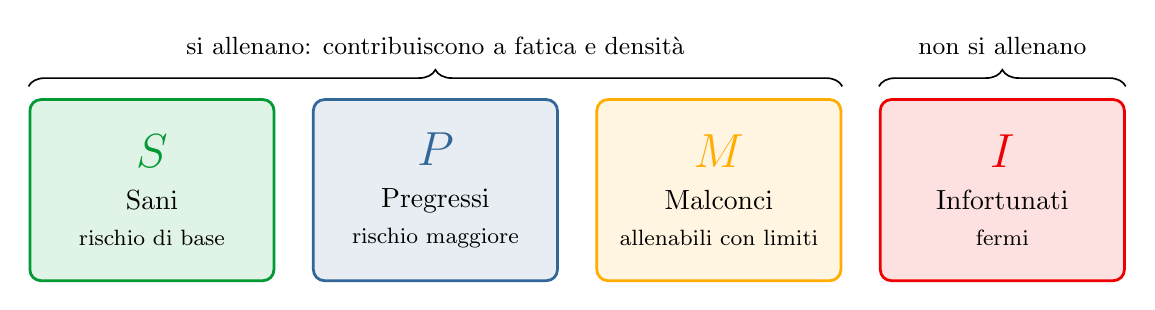
\begin{tikzpicture}[
        population/.style = {
            rectangle, rounded corners = 4pt, line width = 1pt,
            minimum width = 3.1cm, minimum height = 2.3cm, align = center
        }
    ]
        \node[population, draw = ColorS, fill = ColorS!12] (S) at (0, 0)
            {{\LARGE\bfseries\color{ColorS} $S$}\\[3pt] Sani\\[1pt] {\footnotesize rischio di base}};
        \node[population, draw = ColorP, fill = ColorP!12] (P) at (3.6, 0)
            {{\LARGE\bfseries\color{ColorP} $P$}\\[3pt] Pregressi\\[1pt] {\footnotesize rischio maggiore}};
        \node[population, draw = ColorM, fill = ColorM!12] (M) at (7.2, 0)
            {{\LARGE\bfseries\color{ColorM} $M$}\\[3pt] Malconci\\[1pt] {\footnotesize allenabili con limiti}};
        \node[population, draw = ColorI, fill = ColorI!12] (I) at (10.8, 0)
            {{\LARGE\bfseries\color{ColorI} $I$}\\[3pt] Infortunati\\[1pt] {\footnotesize fermi}};

        \draw[decorate, decoration = {brace, amplitude = 6pt}, line width = 0.6pt]
            (S.north west) ++(0, 0.15) -- ($(M.north east) + (0, 0.15)$)
            node[midway, above = 8pt, font = \small] {si allenano: contribuiscono a fatica e densità};
        \draw[decorate, decoration = {brace, amplitude = 6pt}, line width = 0.6pt]
            (I.north west) ++(0, 0.15) -- ($(I.north east) + (0, 0.15)$)
            node[midway, above = 8pt, font = \small] {non si allenano};
    \end{tikzpicture}
    \caption{Le quattro popolazioni del modello}
\end{figure}

La scelta di distinguere quattro popolazioni, invece di due o tre, è motivata dalla necessità di rappresentare separatamente tre aspetti distinti: il rischio di infortunio, che è diverso per sani, pregressi e malconci; la capacità di allenarsi, che distingue gli infortunati dagli altri; il recupero parziale, che non riporta l'atleta allo stato di sano ma lo rende nuovamente allenabile. Se avessimo distinto solo sani e infortunati, non avremmo potuto differenziare il rischio tra sani e pregressi, né modellare il recupero parziale. Se avessimo distinto solo tre popolazioni, avremmo dovuto rinunciare a una di queste distinzioni, con una perdita di realismo. \par

Le popolazioni $S$, $P$, $I$, $M$ sono rappresentate come numeri reali non negativi, non come conteggi interi. Questa scelta è giustificata dal fatto che il modello è pensato per gruppi sufficientemente numerosi, per i quali le fluttuazioni sono trascurabili e l'approssimazione continua è adeguata.

\subsection{Accumulo di fatica}

A queste popolazioni si aggiungono due variabili di stato che descrivono l'accumulo di fatica negli atleti:
\begin{itemize}
    \item Fatica fisica del gruppo $\bar{F}_f$: rappresenta il livello medio di affaticamento muscolare e articolare del gruppo che si allena. Aumenta con il carico di allenamento e diminuisce con il recupero.
    \item Fatica psicologica del gruppo $\bar{F}_p$: rappresenta il livello medio di affaticamento mentale del gruppo che si allena. Aumenta con il carico di allenamento e con lo stress legato alla competizione, e diminuisce con il recupero.
\end{itemize}

\begin{figure}[ht]
    \centering
    \includegraphics[width = 0.8\textwidth]{pictures/post-randori.jpeg}
    \caption[Atleti al termine di un allenamento]{Atleti al termine di una seduta di randori}
\end{figure}

Le due componenti della fatica sono trattate separatamente perché evolvono con dinamiche proprie e contribuiscono in modo distinto al rischio di infortunio. Un atleta può essere fisicamente fresco ma mentalmente affaticato, o viceversa. La separazione permette di modellare scenari in cui il carico fisico e quello psicologico non sono proporzionali, e di studiare l'effetto di ciascuna componente sul rischio complessivo. Inoltre, le due componenti possono avere tassi di recupero diversi, e la loro separazione permette di catturare questa differenza senza forzare una relazione di proporzionalità tra fatica fisica e psicologica. \par

La fatica è calcolata come media sul gruppo che si allena, cioè sugli atleti in $S$, $P$ e $M$. Gli atleti in $I$ non contribuiscono al calcolo, perché non si allenano e non sono esposti al carico. Questa scelta riflette il fatto che la fatica rilevante per il rischio di infortunio è quella degli atleti che effettivamente partecipano all'allenamento. Se gli atleti infortunati contribuissero alla media, la fatica media risulterebbe artificialmente diluita, perché gli infortunati sono per definizione a riposo. \par

Le variabili $\bar{F}_f$ e $\bar{F}_p$ sono rappresentate come numeri reali non negativi. La loro evoluzione è descritta da equazioni che bilanciano il carico aggiunto in ogni seduta e il recupero nel tempo. In ogni passo $t \to t+1$, il gruppo accumula una quantità di fatica proporzionale al carico della seduta, e ne smaltisce una parte proporzionale al livello di fatica corrente. Questa descrizione riprende, in forma semplificata, l'idea dei modelli di risposta all'allenamento proposti da Banister e collaboratori, in cui ogni seduta produce un effetto di fatica che si riduce progressivamente nel tempo, noti come modelli fitness-fatica~\cite{imbach2022}.

\begin{figure}[ht]
    \centering
    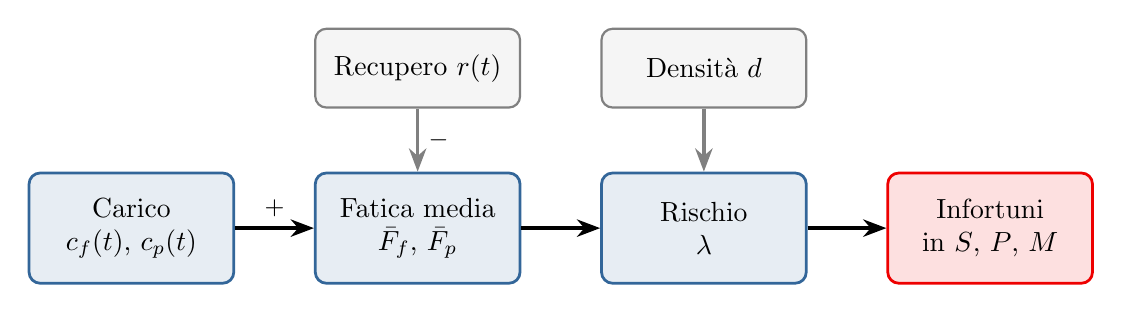
\begin{tikzpicture}[
        block/.style = {
            rectangle, rounded corners = 4pt, draw = ColorP, line width = 1pt, fill = ColorP!12,
            minimum width = 2.6cm, minimum height = 1.4cm, align = center
        },
        input/.style = {
            rectangle, rounded corners = 4pt, draw = gray, line width = 0.8pt, fill = gray!8,
            minimum width = 2.6cm, minimum height = 1cm, align = center
        },
        flow/.style = {-Stealth, line width = 1.2pt}
    ]
        \node[block] (load) {Carico\\ $c_f(t)$, $c_p(t)$};
        \node[block, right = 1cm of load] (fatigue) {Fatica media\\ $\bar{F}_f$, $\bar{F}_p$};
        \node[block, right = 1cm of fatigue] (risk) {Rischio\\ $\lambda$};
        \node[block, draw = ColorI, fill = ColorI!12, right = 1cm of risk] (injuries) {Infortuni\\ in $S$, $P$, $M$};

        \node[input, above = 0.8cm of fatigue] (recovery) {Recupero $r(t)$};
        \node[input, above = 0.8cm of risk] (density) {Densità $d$};

        \draw[flow] (load) -- node[above, font = \small] {$+$} (fatigue);
        \draw[flow] (fatigue) -- (risk);
        \draw[flow] (risk) -- (injuries);
        \draw[flow, draw = gray] (recovery) -- node[right, font = \small] {$-$} (fatigue);
        \draw[flow, draw = gray] (density) -- (risk);
    \end{tikzpicture}
    \caption{Dal carico di allenamento agli infortuni: il ruolo della fatica}
\end{figure}

\section{Ipotesi iniziali}

Per garantire la coerenza e la non distorsione del modello, richiediamo una serie di ipotesi iniziali che non dipendono dalla struttura delle equazioni. Queste ipotesi definiscono il contesto in cui il modello è valido e delimitano le situazioni in cui le sue conclusioni possono essere applicate. \par

In primis, essendo il tempo calcolato in modo discreto $t = 0, 1, \dots, T$, si suppone che le sedute di allenamento siano distribuite equidistanti nel tempo, così che ogni passo del modello $t \to t+1$ abbia approssimativamente la stessa lunghezza. Questo viene richiesto per poter calcolare correttamente la decadenza della fatica accumulata: se gli intervalli tra le sedute fossero di lunghezza diversa, il recupero tra due passi consecutivi non sarebbe confrontabile, e la dinamica della fatica risulterebbe distorta. L'ipotesi di equidistanza permette di trattare il tempo come una variabile regolare e di utilizzare le stesse funzioni di recupero per ogni passo. Un eventuale giorno di riposo, cioè una seduta di allenamento saltata, può essere considerato come una seduta a carico di fatica nullo e trattato all'interno delle variabili di accumulo della fatica, senza bisogno di modificare la struttura del modello. \par

Per poter considerare gli atleti come gruppo e non come singoli individui, sia in termini di accumulo di fatica sia di probabilità di infortunio, supponiamo che abbiano una preparazione fisica e tecnica omogenea, quindi che non ci siano differenze marcate tra di loro. Questa ipotesi è necessaria per giustificare l'uso di variabili medie, cioè $\bar{F}_f$ e $\bar{F}_p$, al posto delle fatiche individuali e per poter applicare lo stesso tasso di infortunio a tutti gli atleti di una data popolazione. Se il gruppo fosse eterogeneo, la media non sarebbe rappresentativa e il modello perderebbe di significato. L'omogeneità non richiede che gli atleti siano identici, ma che le differenze siano trascurabili rispetto alla scala dei fenomeni modellati. \par

L'orizzonte temporale è breve, ad esempio una settimana, un mese o una stagione sportiva. Questo fa sì che gli atleti infortunati $I$ o malconci $M$ non abbiano sufficiente tempo di recuperare completamente e tornare nella popolazione $P$ o $S$. Di conseguenza, nel modello è previsto un solo percorso di recupero, quello da infortunati $I$ a malconci $M$, che rappresenta una guarigione parziale. Il ritorno completo allo stato di sano o di pregresso è escluso perché richiederebbe tempi più lunghi di quelli considerati. Questa ipotesi semplifica la struttura del modello e riflette la realtà di un periodo di allenamento, in cui gli infortuni gravi raramente si risolvono completamente prima della fine del periodo. \par

Le popolazioni sono numeri reali, non conteggi interi. Il modello quindi è significativo e non distorto se il numero di atleti è sufficientemente numeroso. Questa ipotesi permette di evitare le complicazioni legate alla discretizzazione dei conteggi. Per gruppi piccoli, le fluttuazioni potrebbero diventare rilevanti e l'approssimazione continua potrebbe perdere accuratezza, ma per gruppi sufficientemente numerosi le dinamiche aggregate sono ben descritte dal modello continuo. \par

\subsection{Ipotesi sulla fatica media}\label{sec:ipotesi-fatica}

Il modello non descrive la fatica di ogni singolo atleta, ma soltanto la fatica media del gruppo, e usa questa media per calcolare il rischio di infortunio di tutti gli atleti. Questa semplificazione richiede alcune ipotesi aggiuntive, che riguardano il modo in cui gli atleti si allenano insieme sul tatami. \par

La prima è l'ipotesi di mescolamento. Durante l'allenamento di judo gli atleti lavorano a coppie, e nel corso di una seduta le coppie cambiano spesso: nel randori, ad esempio, ogni atleta combatte con molti compagni diversi. Supponiamo che questi cambi avvengano frequentemente e in modo casuale, così che ogni atleta, nel corso della seduta, incontri compagni che nel complesso rappresentano bene l'intero gruppo. In questo modo la fatica dei compagni con cui un atleta si allena è, in media, uguale alla fatica media del gruppo, e ha senso usare $\bar{F}_f$ e $\bar{F}_p$ al posto delle fatiche individuali. Se invece le coppie fossero fisse, ad esempio sempre gli stessi due atleti per tutta la seduta, la fatica rilevante sarebbe quella della singola coppia e la media del gruppo non basterebbe a descriverla. \par

\begin{figure}[ht]
    \centering
    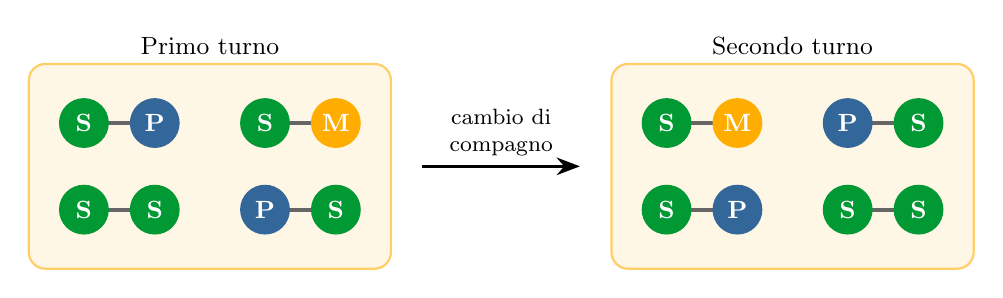
\begin{tikzpicture}[
        athlete/.style = {circle, minimum size = 18pt, inner sep = 0pt, text = white, font = \bfseries\small},
        partner/.style = {line width = 1.5pt, draw = black!60},
        tatami/.style = {rounded corners = 6pt, fill = ColorM!10, draw = ColorM!60, line width = 0.8pt}
    ]
        \newcommand{\pair}[4]{%
            \draw[partner] (#1 - 0.45, #2) -- (#1 + 0.45, #2);
            \node[athlete, fill = Color#3] at (#1 - 0.45, #2) {#3};
            \node[athlete, fill = Color#4] at (#1 + 0.45, #2) {#4};
        }

        % primo turno
        \draw[tatami] (0, 0) rectangle (4.6, 2.6);
        \node[above, font = \small] at (2.3, 2.6) {Primo turno};
        \pair{1.15}{1.85}{S}{P}
        \pair{3.45}{1.85}{S}{M}
        \pair{1.15}{0.75}{S}{S}
        \pair{3.45}{0.75}{P}{S}

        % cambio di compagno
        \draw[-Stealth, line width = 1.2pt] (5, 1.3) -- node[above, font = \footnotesize, align = center] {cambio di\\compagno} (7, 1.3);

        % secondo turno
        \draw[tatami] (7.4, 0) rectangle (12, 2.6);
        \node[above, font = \small] at (9.7, 2.6) {Secondo turno};
        \pair{8.55}{1.85}{S}{M}
        \pair{10.85}{1.85}{P}{S}
        \pair{8.55}{0.75}{S}{P}
        \pair{10.85}{0.75}{S}{S}
    \end{tikzpicture}
    \caption{Ipotesi di mescolamento: le coppie cambiano spesso durante la seduta}
\end{figure}


La seconda è l'ipotesi di simmetria. In uno sport di contatto un infortunio non dipende soltanto dalla stanchezza di chi si infortuna: un atleta riposato può farsi male perché il compagno, stanco, esegue male una tecnica o non controlla una caduta. Supponiamo quindi che il rischio dipenda dalla fatica dell'incontro nel suo insieme, cioè di entrambi gli atleti, e non solo da quella del singolo. Anche questa ipotesi porta a usare la fatica media del gruppo: ciò che conta è quanto è stanco in media chi si trova sul tatami, e non chi in particolare si infortuna. \par

La terza riguarda il gruppo su cui si calcola la media. La fatica media è calcolata soltanto sugli atleti che si allenano, cioè sulle popolazioni $S$, $P$ e $M$, perché gli infortunati in $I$ sono fermi e non partecipano agli incontri. Supponiamo inoltre che l'evoluzione della fatica media non dipenda dai cambiamenti nella composizione del gruppo: quando un atleta si infortuna, abbandona o si aggiunge al gruppo, la fatica media degli altri non cambia per questo motivo. È una semplificazione ragionevole se il gruppo è numeroso, perché l'ingresso o l'uscita di pochi atleti sposta di poco la media. \par

Queste ipotesi, insieme a quelle di omogeneità e di numerosità del gruppo discusse sopra, giustificano l'uso delle fatiche medie al posto delle fatiche individuali e permettono al modello di descrivere in modo adeguato le dinamiche collettive del gruppo.

\subsection{Ipotesi sugli infortuni e sulle transizioni}

Le equazioni del modello descrivono gli infortuni e i passaggi tra le popolazioni attraverso tassi e probabilità. Questo richiede alcune ipotesi su come avvengono gli infortuni durante una seduta e su come gli atleti cambiano popolazione. \par

La prima riguarda l'indipendenza degli infortuni. Supponiamo che, all'interno di una seduta, ogni atleta si infortuni indipendentemente dagli altri, con una probabilità che dipende soltanto dalla sua popolazione, dalla fatica media del gruppo e dalla densità sul tatami. Per questo motivo il numero di infortuni di una popolazione è proporzionale al numero di atleti che la compongono. In questo modo il legame tra gli atleti viene descritto solo attraverso le grandezze medie del gruppo, come previsto dalle ipotesi sulla fatica media. \par

La seconda riguarda la gravità dell'infortunio. Supponiamo che la probabilità $\pi$ che un infortunio sia grave sia la stessa per tutte le popolazioni. Un atleta più a rischio, come un malconcio, si infortuna più spesso, ma quando si infortuna la gravità dell'infortunio non dipende dalla popolazione di provenienza. \par

La terza riguarda l'esposizione al rischio. Supponiamo che in ogni seduta tutti gli atleti che possono allenarsi, cioè quelli in $S$, $P$ e $M$, siano esposti al rischio di infortunio, qualunque sia il carico della seduta. Il carico influenza il rischio soltanto attraverso la fatica accumulata: anche una seduta a carico nullo, come una seduta leggera o di scarico, comporta quindi un rischio, dovuto alla fatica residua e alla densità sul tatami. Se in un giorno gli atleti non si allenassero affatto, il modello sovrastimerebbe gli infortuni di quel giorno. \par

La quarta riguarda l'ordine degli eventi nella seduta. Supponiamo che gli abbandoni, gli infortuni e i recuperi di una seduta avvengano tutti a partire dalle popolazioni all'inizio della seduta, cioè al passo $t$, e producano i loro effetti al passo $t+1$. Un atleta, quindi, non può infortunarsi e abbandonare nella stessa seduta: per questo motivo, affinché le popolazioni restino non negative, la somma dei tassi di uscita da ciascuna popolazione non deve superare $1$. \par

La quinta riguarda l'assenza di memoria. Supponiamo che la probabilità di passare da una popolazione all'altra dipenda soltanto dalla popolazione in cui si trova l'atleta, e non da quanto tempo vi si trova. In particolare, un infortunato grave torna allenabile con la stessa probabilità $\rho$ in ogni seduta, indipendentemente da quando si è infortunato. Il tempo passato in $I$ è quindi casuale, con media pari a $1 / \rho$ sedute: alcuni atleti tornano ad allenarsi presto, altri molto più tardi. Nella realtà la durata di un infortunio dipende dal tipo di lesione, ma questa ipotesi permette di descrivere il recupero con un solo parametro. \par

L'ultima riguarda il recupero dalla fatica. Supponiamo che il tasso di recupero $r$ dipenda dal tempo e non dalla fatica del gruppo. La funzione $r(t)$ rappresenta la capacità del gruppo di smaltire la fatica tra una seduta e la successiva, che si riduce con il protrarsi del periodo di allenamento per effetto della stanchezza che si accumula sulle settimane, del sonno e degli impegni esterni. La fatica della singola seduta, invece, è già descritta dalla variabile $\bar{F}_\cdot$, e la quantità smaltita è proporzionale ad essa. È una semplificazione: in un modello più dettagliato il recupero potrebbe dipendere anche dal livello di fatica raggiunto.

\section{Condizioni iniziali}

Le condizioni iniziali del modello sono:
\begin{itemize}
    \item $S(0) \geq 0$: il gruppo può iniziare con un numero arbitrario di atleti sani.
    \item $P(0) \geq 0$: il gruppo può iniziare con un numero arbitrario di atleti con infortuni pregressi.
    \item $I(0) = 0$: si assume che nessun atleta sia infortunato all'inizio del periodo considerato.
    \item $M(0) = 0$: si assume che nessun atleta sia malconcio all'inizio del periodo considerato.
    \item $\bar{F}_f(0) \geq 0$: la fatica fisica può essere presente all'inizio del periodo considerato, ma si preferisce considerarla nulla.
    \item $\bar{F}_p(0) \geq 0$: la fatica psicologica può essere presente all'inizio del periodo considerato, ma si preferisce considerarla nulla.
\end{itemize}
Si deve avere inoltre che $S(0) + P(0) > 0$, cioè che la popolazione iniziale non sia vuota. Senza atleti sani o con infortuni pregressi, il modello non avrebbe una popolazione di partenza su cui evolvere, e le equazioni perderebbero di significato. La condizione $I(0) = M(0) = 0$ è invece una scelta semplificativa, non un requisito di coerenza. \par

La scelta $I(0) = M(0) = 0$ è coerente con l'idea che il modello descriva un periodo di allenamento che inizia in condizioni di relativa normalità, senza infortuni in corso. Se il periodo considerato iniziasse immediatamente dopo un infortunio, o in una fase di recupero, sarebbe più appropriato porre $I(0) > 0$ e $M(0) > 0$. In questa prima formulazione si assume che il gruppo parta da una condizione di salute, e che eventuali infortuni siano il risultato dell'evoluzione del modello, non una condizione iniziale.

Le condizioni iniziali su $\bar{F}_f(0)$ e $\bar{F}_p(0)$ ammettono un livello di fatica non nullo all'inizio, ma si preferisce considerarlo nullo. In questo modo si suppone che il gruppo parta da uno stato di freschezza, eventualmente dopo un periodo di riposo o all'inizio della stagione. Questa scelta semplifica il problema di dover calcolare il livello di fatica medio prima dell'arrivo, e riflette l'ipotesi che il periodo considerato inizi dopo una fase di recupero sufficiente a smaltire la fatica accumulata in precedenza. Condizioni iniziali diverse possono essere considerate per modellare scenari in cui il gruppo entra nel periodo di allenamento con fatica residua, ma in questa prima formulazione si assume che la fatica iniziale sia nulla.

La scelta di porre $\bar{F}_f(0) = \bar{F}_p(0) = 0$ non è obbligatoria, ma è conveniente per due motivi. In primo luogo, semplifica l'analisi del modello, eliminando la necessità di stimare la fatica iniziale del gruppo. In secondo luogo, rende più chiari i confronti tra scenari diversi, perché tutti partono dallo stesso stato di freschezza. Se si volesse modellare un gruppo che entra nel periodo con fatica residua, basterebbe porre $\bar{F}_f(0) > 0$ e/o $\bar{F}_p(0) > 0$, senza modificare la struttura delle equazioni.

La scelta di porre $S(0) \geq 0$ e $P(0) \geq 0$, con $S(0) + P(0) > 0$, riflette il fatto che il gruppo può iniziare con una composizione arbitraria di atleti sani e con infortuni pregressi. Il modello non richiede che tutti gli atleti siano sani, né che tutti abbiano infortuni pregressi. La composizione iniziale è un parametro del modello, che può essere variato per studiare scenari diversi.

\section{Funzioni}

Nelle equazioni del modello sono presenti cinque funzioni, che regolano i processi di ingresso, uscita, infortunio, carico e recupero. Esse costituiscono il legame tra i parametri e la dinamica delle variabili di stato, e la loro specificazione è necessaria per poter simulare e analizzare il modello.

\begin{itemize}
    \item Funzione di crescita $\mu$: descrive il numero di nuovi atleti che entrano nel gruppo complessivo in ogni seduta. Riflette le dinamiche di iscrizione a una stagione sportiva, con ingressi tipicamente concentrati all'inizio del periodo e progressivamente decrescenti. La funzione dipende dalla frazione di tempo trascorsa e da parametri che ne controllano l'ampiezza e la forma.
    \item Funzione di abbandono $\nu$: descrive la frazione di atleti che abbandona il gruppo in ogni seduta, per motivi diversi. Il suo profilo temporale può essere opposto a quello della funzione di crescita, dato che gli abbandoni tendono a concentrarsi alla fine del periodo, quando l'entusiasmo iniziale si riduce o sopraggiungono altri impegni. La funzione è modulata da un moltiplicatore specifico per la popolazione a cui si applica.
    \item Funzione di infortunio $\lambda$: descrive la probabilità che un atleta si infortuni in una seduta. Dipende dalla fatica fisica e psicologica media del gruppo, dalla densità di atleti sul tatami e da un moltiplicatore di rischio specifico per la popolazione a cui è applicata. La funzione è crescente rispetto a fatica e densità e si satura a un valore massimo.
    \item Funzione di carico $c$: fornisce il tasso di carico di ogni seduta di allenamento per le due componenti della fatica, fisica e psicologica. Può essere costante, periodica o variabile nel tempo, e rappresenta l'entrata principale che determina l'accumulo di fatica.
    \item Funzione di recupero $r$: descrive il tasso di smaltimento della fatica in ogni seduta. Il recupero può essere massimo all'inizio del periodo, quando gli atleti sono freschi, e decrescere nel tempo, man mano che la fatica si accumula.
\end{itemize}

Queste funzioni verranno specificate in dettaglio più avanti, dove verranno definite le loro forme analitiche, i parametri, i domini e le proprietà. In questa sede è sufficiente averne un'idea qualitativa: $\mu$ e $\nu$ regolano i flussi di popolazione, $\lambda$ regola il rischio di infortunio, $c$ fornisce il carico di allenamento e $r$ regola la dinamica della fatica. Le loro interazioni determinano l'evoluzione del sistema e la composizione del gruppo nel tempo.
    \chapter{Modello senza controllo}

\section{Equazione di S}

La popolazione $S$ descrive l'evoluzione degli atleti sani, cioè coloro che non hanno infortuni in corso né infortuni pregressi. Gli atleti in questa popolazione si allenano senza limitazioni e sono considerati il gruppo di riferimento per il rischio di infortunio. La dinamica è descritta dalla seguente equazione:
\begin{align*}
    S(t+1) &= S(t) \\
        &+ \alpha \mu\left(\frac{t}{T}\right) \\
        &- \nu\left(\frac{t}{T}, \beta_S\right) S(t) \\
        &- \lambda\left(\bar{F}_f(t), \bar{F}_p(t), \frac{S(t) + P(t) + M(t)}{A_{\max}}, \gamma_S\right) S(t)
\end{align*}

L'equazione ha la struttura comune a tutte le equazioni del modello: la popolazione al passo successivo è uguale alla popolazione corrente, più i flussi in ingresso, meno i flussi in uscita. Nel caso di $S$, i flussi sono tre, cioè un ingresso, un'uscita per abbandono e un'uscita per infortunio. Questa struttura garantisce che la popolazione al passo successivo sia determinata dalla popolazione corrente e dai flussi che la attraversano, senza dipendenze dirette da altre variabili di stato se non attraverso le funzioni $\mu$, $\nu$ e $\lambda$. La scelta di scrivere l'equazione in questa forma, invece che in forma compatta, permette di identificare immediatamente il ruolo di ciascun termine e di verificare la coerenza dei flussi.

\paragraph{Flusso di ingresso}
Il termine
\[
    \alpha \mu\left(\frac{t}{T}\right)
\]
rappresenta il flusso di nuovi atleti che entrano nel gruppo e sono sani. La funzione $\mu$ descrive il numero complessivo di nuovi ingressi alla frazione di tempo $t/T$. Le sue caratteristiche specifiche, come quelle delle altre funzioni del modello, verranno esposte in seguito. In questa sede è sufficiente sapere che $\mu$ è una funzione non negativa del tempo, che riflette la dinamica di iscrizione a una stagione sportiva. \\
La frazione $\alpha \in [0,1]$ rappresenta la quantità di atleti nuovi che è sana, mentre i restanti entrano nella popolazione $P$. La scelta di distribuire gli ingressi tra sani e pregressi riflette il fatto che non tutti i nuovi atleti sono in condizioni ottimali: alcuni hanno già avuto infortuni pregressi e vengono quindi classificati in $P$. La distribuzione è controllata dal parametro $\alpha$, che può essere calibrato in base alla composizione attesa del gruppo. \par

In questo caso la variazione è assoluta, cioè il numero di atleti che entrano non dipende dal valore della popolazione corrente né dalle altre popolazioni. Questa scelta riflette il fatto che gli ingressi sono determinati da fattori esterni al modello, come iscrizioni, trasferimenti e arrivi programmati, e non dalla dinamica interna del gruppo. Un'eventuale dipendenza degli ingressi dalla dimensione del gruppo potrebbe essere introdotta in estensioni future, ad esempio per modellare il passaparola o la capacità ricettiva della palestra, ma in questa prima formulazione si assume che $\mu$ sia una funzione dipendente solo dal tempo. La scelta di un flusso assoluto, invece che di un tasso pro capite, è coerente con il fatto che gli ingressi sono eventi esterni e non dipendono dallo stato del gruppo.

\paragraph{Flusso di abbandono}
Il termine
\[
    \nu\left(\frac{t}{T}, \beta_S\right) S(t)
\]
rappresenta il flusso di atleti sani che abbandonano il gruppo. La funzione $\nu$ è il tasso di abbandono pro capite, modulato dal parametro $\beta_S$ specifico della popolazione $S$. Nell'equazione di $S$, gli abbandoni sono dovuti a motivi diversi dall'infortunio, come trasferimenti, perdita di interesse, impegni personali, cambi di attività e partenze anticipate. Questi motivi sono distinti da quelli che portano all'infortunio, che sono modellati separatamente dal termine $\lambda$. La distinzione è importante perché i due fenomeni hanno cause diverse e dinamiche diverse: l'abbandono è una scelta volontaria o comunque esterna all'allenamento, mentre l'infortunio è un evento che avviene durante l'allenamento ed è influenzato dal carico e dalla fatica. \par

Generalmente la funzione di crescita è approssimativamente decrescente. Un atleta può aggiungersi in ritardo, ad esempio per motivi logistici come trasporti per raggiungere uno stage o altre attività obbligatorie, quindi più il tempo avanza, più è improbabile che un atleta si inserisca. Al contrario, è difficile che un atleta abbandoni già dopo il primo allenamento, mentre più ci si avvicina alla fine del periodo, più è probabile che un atleta se ne vada prima, ad esempio perché ha un mezzo di trasporto da prendere per tornare a casa, oppure perché ha raggiunto la saturazione di stanchezza. \\
Quindi il profilo temporale della funzione $\nu$ può essere l'opposto rispetto a quello della funzione $\mu$: gli ingressi si concentrano all'inizio e gli abbandoni alla fine. Questa opposizione non è un requisito del modello, ma una scelta di modellazione che riflette l'esperienza tipica di una stagione sportiva. \par

Il fatto che $\nu$ dipenda dal tempo e non dallo stato riflette l'ipotesi che gli abbandoni siano determinati da fattori esterni al modello, come la stagionalità, la durata del periodo o eventi personali, e non dalla dinamica interna del gruppo. In estensioni future, si potrebbe considerare una dipendenza di $\nu$ dalla fatica o dalla soddisfazione degli atleti, ma in questa prima formulazione si assume che $\nu$ sia una funzione dipendente solo dal tempo. La scelta di un tasso pro capite, invece che di un flusso assoluto, è coerente con il fatto che l'abbandono è un evento individuale: ogni atleta ha una certa probabilità di abbandonare indipendentemente dagli altri. Il flusso di abbandono è quindi proporzionale alla popolazione considerata.

\paragraph{Flusso di infortunio}
Il termine
\[
    \lambda\left(\bar{F}_f(t), \bar{F}_p(t), \frac{S(t) + P(t) + M(t)}{A_{\max}}, \gamma_S\right) S(t)
\]
rappresenta il flusso di atleti sani che si infortunano durante la seduta. La funzione $\lambda$ descrive la probabilità di infortunio, che dipende dalla fatica fisica e psicologica media del gruppo, dalla densità sul tatami e dal moltiplicatore di rischio $\gamma_S$, specifico della popolazione $S$. La densità è calcolata come
\[
    \frac{S(t) + P(t) + M(t)}{A_{\max}}
\]
perché gli atleti in $I$ non si allenano e non contribuiscono alla concentrazione sul tatami. La densità riflette il numero di atleti effettivamente presenti sul tatami, normalizzato rispetto a una scala di riferimento $A_{\max}$ che rappresenta la capienza del tatami, cioè il numero massimo di atleti che possono allenarsi in sicurezza. Più atleti ci sono sul tatami, più è probabile che si verifichino scontri tra coppie, impatti o contatti accidentali, e quindi più alto è il rischio di infortunio. \par

Gli atleti che si infortunano escono da $S$ ed entrano in $I$ o $M$, a seconda che l'infortunio sia grave, con probabilità $\pi$, o meno grave, con probabilità $1-\pi$. Questa transizione è descritta nelle equazioni di $I$ e $M$. Il fatto che il flusso di infortunio sia proporzionale a $S(t)$ riflette l'ipotesi che ogni atleta sano abbia la stessa probabilità di infortunarsi, indipendentemente dagli altri. La probabilità dipende dalla fatica media, che riflette lo stato complessivo degli atleti che si allenano, e dalla densità, che riflette la concentrazione di atleti sul tatami. La scelta di usare la fatica media, invece delle fatiche individuali, è giustificata dalle ipotesi di mescolamento e simmetria discusse nel capitolo precedente: gli accoppiamenti cambiano frequentemente e ogni atleta interagisce in media con partner rappresentativi della fatica media del gruppo.

\section{Equazione di P}

La popolazione $P$ descrive l'evoluzione degli atleti con infortuni pregressi, cioè coloro che hanno avuto infortuni prima dell'inizio del periodo considerato e che, pur essendo pienamente allenabili, sono considerati più a rischio rispetto agli atleti sani. La dinamica è descritta dall'equazione:
\begin{align*}
    P(t+1) &= P(t) \\
        &+ (1 - \alpha) \mu\left(\frac{t}{T}\right) \\
        &- \nu\left(\frac{t}{T}, \beta_P\right) P(t) \\
        &- \lambda\left(\bar{F}_f(t), \bar{F}_p(t), \frac{S(t) + P(t) + M(t)}{A_{\max}}, \gamma_P\right) P(t)
\end{align*}

L'equazione ha la stessa struttura dell'equazione di $S$: la popolazione al passo successivo è uguale alla popolazione corrente, più i flussi in ingresso, meno i flussi in uscita. Nel caso di $P$, i flussi sono sempre tre, cioè un ingresso, un'uscita per abbandono e un'uscita per infortunio. La differenza rispetto a $S$ sta nei parametri e nel tipo di atleti che la popolazione raccoglie. La scelta di mantenere la stessa struttura per le due equazioni semplifica la scrittura del sistema completo e facilita il confronto tra le popolazioni.

\paragraph{Flusso di ingresso}
Il termine
\[
    (1 - \alpha) \mu\left(\frac{t}{T}\right)
\]
rappresenta il flusso di nuovi atleti che entrano nel gruppo e hanno infortuni pregressi. La funzione $\mu$ descrive il numero complessivo di nuovi ingressi alla frazione di tempo $t/T$, come nell'equazione di $S$. Come già descritto, la frazione $1 - \alpha \in [0,1]$ rappresenta la quantità di atleti nuovi che ha infortuni pregressi. \\
La somma dei due flussi di ingresso è
\[
    \alpha\mu + (1-\alpha)\mu = \mu
\]
coerente con il fatto che tutti i nuovi ingressi sono distribuiti tra $S$ e $P$. La scelta di distribuire gli ingressi tra le due popolazioni, invece di assegnarli tutti a $S$, riflette il fatto che una parte dei nuovi atleti ha una storia clinica pregressa e non può essere considerata pienamente sana.

\paragraph{Flusso di abbandono}
Il termine
\[
    \nu\left(\frac{t}{T}, \beta_P\right) P(t)
\]
rappresenta il flusso di atleti con infortuni pregressi che abbandonano il gruppo. La funzione $\nu$ è il tasso di abbandono pro capite, questa volta modulato dal parametro $\beta_P$ specifico della popolazione $P$. Anche in questo caso, gli abbandoni sono dovuti a motivi diversi dall'infortunio, come trasferimenti, perdita di interesse, impegni personali, cambi di attività e partenze anticipate. Il profilo temporale di $\nu$ può essere lo stesso di quello usato per $S$, ma il parametro $\beta_P$ permette di differenziare il tasso di abbandono tra le due popolazioni. \par

La scelta di introdurre un parametro $\beta_P$ distinto da $\beta_S$ riflette il fatto che gli atleti con infortuni pregressi possono avere un comportamento di abbandono diverso rispetto agli atleti sani. Ad esempio, un atleta con un infortunio pregresso potrebbe essere più propenso ad abbandonare se il carico di allenamento è elevato, perché il rischio di recidiva è maggiore oppure non riesce a sostenere il carico di allenamento. Il parametro $\beta_P$ permette di catturare queste differenze senza modificare la forma della funzione $\nu$. Se non ci fossero differenze attese, si potrebbe porre $\beta_P = \beta_S$ e ricondursi al caso di un tasso di abbandono unico.

\paragraph{Flusso di infortunio}
Il termine
\[
    \lambda\left(\bar{F}_f(t), \bar{F}_p(t), \frac{S(t) + P(t) + M(t)}{A_{\max}}, \gamma_P\right) P(t)
\]
rappresenta il flusso di atleti con infortuni pregressi che si infortunano durante la seduta. La funzione $\lambda$ descrive la probabilità di infortunio, come per $S$. La differenza rispetto a $S$ sta nel moltiplicatore di rischio $\gamma_P$. Gli atleti con infortuni pregressi sono considerati più a rischio rispetto agli atleti sani, in quanto un infortunio pregresso può lasciare una vulnerabilità residua, una ridotta stabilità articolare o una minore tolleranza al carico. Questo si riflette nell'ipotesi di lavoro $\gamma_S \leq \gamma_P$, riportata in \autoref{sec:domini}. Il parametro $\gamma_P$ permette quindi di calibrare il rischio aggiuntivo associato agli infortuni pregressi. Se, ad esempio, si ritiene che un atleta con infortunio pregresso abbia un rischio doppio rispetto a un atleta sano, si può porre $\gamma_P = 2\gamma_S$. \par

Come per $S$, gli atleti che si infortunano escono da $P$ ed entrano in $I$ o $M$, a seconda che l'infortunio sia grave o meno grave. Questa transizione è descritta nelle equazioni di $I$ e $M$. Il fatto che il flusso di infortunio sia proporzionale a $P(t)$ riflette l'ipotesi che ogni atleta con infortunio pregresso abbia la stessa probabilità di infortunarsi, indipendentemente dagli altri. La probabilità è modulata dalla fatica media del gruppo e dalla densità, come per $S$.

\section{Equazione di I}

La popolazione $I$ descrive l'evoluzione degli atleti infortunati, cioè coloro che si sono infortunati durante il periodo considerato e non si stanno allenando. Questi atleti sono temporaneamente esclusi dall'attività e non contribuiscono alla densità sul tatami. La loro presenza è rilevante perché rappresenta l'esito più grave del rischio di infortunio e perché il loro recupero parziale alimenta la popolazione $M$. La dinamica è descritta dalla seguente equazione:
\begin{align*}
    I(t+1) &= I(t) \\
        &+ \pi \lambda\left(\bar{F}_f(t), \bar{F}_p(t), \frac{S(t) + P(t) + M(t)}{A_{\max}}, \gamma_S\right) S(t) \\
        &+ \pi \lambda\left(\bar{F}_f(t), \bar{F}_p(t), \frac{S(t) + P(t) + M(t)}{A_{\max}}, \gamma_P\right) P(t) \\
        &+ \pi \lambda\left(\bar{F}_f(t), \bar{F}_p(t), \frac{S(t) + P(t) + M(t)}{A_{\max}}, \gamma_M\right) M(t) \\
        &- \rho I(t) \\
        &- \nu\left(\frac{t}{T}, \beta_I\right) I(t)
\end{align*}

L'equazione ha la stessa struttura delle equazioni di $S$, $P$ e $M$: la popolazione al passo successivo è uguale alla popolazione corrente, più i flussi in ingresso, meno i flussi in uscita. Nel caso di $I$, i flussi in ingresso sono tre, uno da ciascuna delle altre popolazioni, mentre i flussi in uscita sono due, cioè il recupero parziale e l'abbandono. La differenza principale rispetto alle altre popolazioni sta nel fatto che $I$ non ha ingressi diretti dalla popolazione esterna, nessun atleta entra in $I$ se non perché si è infortunato gravemente.

\paragraph{Flussi di ingresso}
I termini
\begin{gather*}
    \pi \lambda\left(\bar{F}_f(t), \bar{F}_p(t), \frac{S(t) + P(t) + M(t)}{A_{\max}}, \gamma_S\right) S(t) \\
    \pi \lambda\left(\bar{F}_f(t), \bar{F}_p(t), \frac{S(t) + P(t) + M(t)}{A_{\max}}, \gamma_P\right) P(t) \\
    \pi \lambda\left(\bar{F}_f(t), \bar{F}_p(t), \frac{S(t) + P(t) + M(t)}{A_{\max}}, \gamma_M\right) M(t)
\end{gather*}
rappresentano i flussi di atleti che si infortunano gravemente e provengono rispettivamente da $S$, $P$ e $M$. In tutti e tre i casi la funzione $\lambda$ rappresenta la probabilità di infortunio relativa alla popolazione specificata. La presenza di tre termini distinti riflette il fatto che gli atleti possono infortunarsi indipendentemente dalla popolazione di appartenenza: un atleta sano, un atleta con infortunio pregresso e un atleta malconcio hanno tutti una probabilità positiva di infortunarsi, ma il moltiplicatore di rischio $\gamma_\cdot$ permette di differenziare tale probabilità. \par

Il fattore $\pi \in [0,1]$ rappresenta la probabilità che un infortunio sia grave. Quando un atleta si infortuna, indipendentemente dalla popolazione di provenienza, l'infortunio è grave con probabilità $\pi$ e lieve con probabilità $1-\pi$. Solo gli infortuni gravi portano l'atleta in $I$, mentre gli infortuni lievi portano l'atleta in $M$, come descritto nella relativa equazione. La somma dei flussi in ingresso a $I$ e dei flussi in ingresso a $M$ è uguale al flusso totale di infortuni, coerentemente con il fatto che non c'è dispersione in queste transizioni.

\paragraph{Flusso di recupero}
Il termine
\[
    \rho I(t)
\]
rappresenta il flusso di atleti infortunati che guariscono parzialmente e passano alla popolazione $M$. Il parametro $\rho \in [0,1]$ è il tasso di transizione da $I$ a $M$, cioè rappresenta la frazione di atleti infortunati che, per unità di tempo, torna allenabile con qualche restrizione. \\
La scelta di modellare il recupero come transizione $I \to M$, invece che come ritorno diretto a $P$, è dovuta all'ipotesi che l'orizzonte temporale sia breve e che non ci sia abbastanza tempo per un recupero completo. Un atleta che si infortuna gravemente ha bisogno di un periodo di riposo e riabilitazione, seguito da un periodo di reinserimento graduale. Il passaggio a $M$ rappresenta questo reinserimento: l'atleta non è ancora pienamente guarito, ma può ricominciare ad allenarsi con qualche restrizione.

\paragraph{Flusso di abbandono}
Il termine
\[
    \nu\left(\frac{t}{T}, \beta_I\right) I(t)
\]
rappresenta il flusso di atleti infortunati che abbandonano il gruppo. La funzione $\nu$ è il tasso di abbandono pro capite, modulato dal parametro $\beta_I$ specifico della popolazione $I$. In questo caso, gli abbandoni sono dovuti principalmente all'incapacità di continuare gli allenamenti a causa dell'infortunio, oltre ai motivi già elencati per le altre popolazioni. La scelta di introdurre un parametro $\beta_I$ distinto dagli altri riflette il fatto che gli atleti infortunati possono avere un comportamento di abbandono diverso rispetto agli altri: un atleta con un infortunio grave potrebbe essere più propenso ad abbandonare. Generalmente si suppone che $\beta_I$ sia superiore agli altri $\beta_\cdot$.

\section{Equazione di M}

La popolazione $M$ descrive l'evoluzione degli atleti malconci, cioè coloro che hanno infortuni lievi o che sono parzialmente guariti da un infortunio e possono continuare ad allenarsi con qualche restrizione. Questi atleti partecipano all'allenamento, ma la loro condizione fisica non è ottimale e il loro rischio di incorrere in un nuovo infortunio è considerato maggiore rispetto a quello degli atleti sani. La dinamica è descritta dalla seguente equazione:
\begin{align*}
    M(t+1) &= M(t) \\
        &+ (1 - \pi) \lambda\left(\bar{F}_f(t), \bar{F}_p(t), \frac{S(t) + P(t) + M(t)}{A_{\max}}, \gamma_S\right) S(t) \\
        &+ (1 - \pi) \lambda\left(\bar{F}_f(t), \bar{F}_p(t), \frac{S(t) + P(t) + M(t)}{A_{\max}}, \gamma_P\right) P(t) \\
        &- \pi \lambda\left(\bar{F}_f(t), \bar{F}_p(t), \frac{S(t) + P(t) + M(t)}{A_{\max}}, \gamma_M\right) M(t) \\
        &+ \rho I(t) \\
        &- \nu\left(\frac{t}{T}, \beta_M\right) M(t)
\end{align*}

L'equazione ha la stessa struttura delle equazioni di $S$, $P$ e $I$: la popolazione al passo successivo è uguale alla popolazione corrente, più i flussi in ingresso, meno i flussi in uscita. Nel caso di $M$, i flussi in ingresso sono tre, cioè infortuni lievi da $S$, infortuni lievi da $P$ e recupero parziale da $I$, mentre i flussi in uscita sono due, cioè infortunio grave e abbandono. La differenza principale rispetto a $S$ e $P$ sta nel fatto che $M$ non ha ingressi diretti dalla popolazione esterna, nessun atleta entra in $M$ se non perché si è infortunato lievemente o perché è parzialmente guarito da un infortunio grave.

\paragraph{Flussi di ingresso da infortunio lieve}
I termini
\begin{gather*}
    (1 - \pi) \lambda\left(\bar{F}_f(t), \bar{F}_p(t), \frac{S(t) + P(t) + M(t)}{A_{\max}}, \gamma_S\right) S(t) \\
    (1 - \pi) \lambda\left(\bar{F}_f(t), \bar{F}_p(t), \frac{S(t) + P(t) + M(t)}{A_{\max}}, \gamma_P\right) P(t)
\end{gather*}
rappresentano i flussi di atleti sani e con infortuni pregressi che si infortunano lievemente durante la seduta e passano in $M$. La funzione $\lambda$ descrive la probabilità di infortunio, come nelle equazioni di $S$ e $P$, e il fattore $1 - \pi$, come già spiegato, rappresenta la probabilità che l'infortunio sia lieve invece che grave.

\paragraph{Flusso di recupero da I}
Il termine
\[
    \rho I(t)
\]
rappresenta il flusso di atleti infortunati che guariscono parzialmente e passano da $I$ a $M$. Questo termine è già stato descritto nell'equazione di $I$, dove appare con segno negativo. In $M$ appare con segno positivo, perché rappresenta un ingresso. Il parametro $\rho \in [0,1]$ è il tasso di transizione da $I$ a $M$: rappresenta la frazione di atleti infortunati che, per unità di tempo, torna allenabile con qualche restrizione.

\paragraph{Flusso di uscita per infortunio grave}
Il termine
\[
    \pi \lambda\left(\bar{F}_f(t), \bar{F}_p(t), \frac{S(t) + P(t) + M(t)}{A_{\max}}, \gamma_M\right) M(t)
\]
rappresenta il flusso di atleti malconci che si infortunano gravemente durante la seduta e passano in $I$. La funzione $\lambda$ descrive la probabilità di infortunio, modulata dal moltiplicatore di rischio $\gamma_M$ specifico della popolazione $M$. Il fattore $\pi$ rappresenta la probabilità che l'infortunio sia grave. Il fatto che il flusso di uscita sia proporzionale a $\pi$ riflette il fatto che solo gli infortuni gravi portano l'atleta fuori da $M$, mentre gli infortuni lievi lasciano l'atleta in $M$, perché la sua condizione resta quella di malconcio. \par

La differenza rispetto a $S$ e $P$ sta nel moltiplicatore di rischio $\gamma_M$. Gli atleti malconci sono considerati più a rischio rispetto agli atleti sani e, in genere, anche rispetto agli atleti con infortuni pregressi, perché la loro condizione fisica non è ottimale e possono essere più vulnerabili a nuovi infortuni. Questo si riflette nell'ipotesi di lavoro $\gamma_S \leq \gamma_P \leq \gamma_M$, riportata in \autoref{sec:domini}. Il parametro $\gamma_M$ permette quindi di calibrare il rischio aggiuntivo associato alla condizione di malconcio.

\paragraph{Flusso di abbandono}
Il termine
\[
    \nu\left(\frac{t}{T}, \beta_M\right) M(t)
\]
rappresenta il flusso di atleti malconci che abbandonano il gruppo. La funzione $\nu$ è il tasso di abbandono pro capite, modulato dal parametro $\beta_M$ specifico della popolazione $M$. Il parametro $\beta_M$ permette di differenziare il tasso di abbandono dei malconci rispetto a quello delle altre popolazioni: un atleta malconcio potrebbe essere più propenso ad abbandonare se la condizione di disagio persiste.

\section{Equazioni per l'accumulo della fatica}

Le variabili $\bar{F}_f$ e $\bar{F}_p$ descrivono, rispettivamente, l'evoluzione della fatica fisica e psicologica media del gruppo che si allena, cioè degli atleti in $S$, $P$ e $M$. La dinamica delle due componenti è descritta dalle seguenti equazioni:
\begin{align*}
    \bar{F}_f(t+1) &= \bar{F}_f(t)
        + c_f(t)
        - r(t) \bar{F}_f(t) \\[5pt]
    \bar{F}_p(t+1) &= \bar{F}_p(t)
        + c_p(t)
        - r(t) \bar{F}_p(t)
\end{align*}

Le due equazioni hanno la stessa struttura: la fatica al passo successivo è uguale alla fatica corrente, più il carico della seduta, meno la parte di fatica smaltita dal recupero. La differenza tra le due componenti sta nel carico, cioè $c_f$ per la fatica fisica e $c_p$ per quella psicologica, e nei valori iniziali. La struttura identica permette di trattare le due componenti in modo uniforme nell'analisi del modello. La scelta di separare le due componenti riflette il fatto che la fatica fisica e quella psicologica evolvono con dinamiche proprie e contribuiscono in modo distinto al rischio di infortunio.

\paragraph{Carico della seduta}
Il termine $c_f(t)$ rappresenta il carico fisico della seduta al tempo $t$, mentre $c_p(t)$ rappresenta il carico psicologico. Le due funzioni sono parametri esogeni, assegnati dall'esterno, e possono essere costanti, periodiche o variabili nel tempo. Il carico rappresenta la quantità di fatica aggiunta in una singola seduta: non è un tasso, ma un flusso assoluto. Ogni seduta aggiunge $c_f(t)$ alla fatica fisica e $c_p(t)$ alla fatica psicologica, indipendentemente dal livello di fatica corrente. \par

La scelta di modellare il carico come flusso assoluto, invece che come tasso pro capite, riflette il fatto che il carico di una seduta è determinato dall'allenamento programmato, non dallo stato di affaticamento dell'atleta. Se il carico fosse proporzionale alla fatica corrente, un atleta molto affaticato riceverebbe un carico maggiore, il che è irrealistico: in genere l'allenatore riduce il carico quando gli atleti sono affaticati, oppure lo mantiene costante indipendentemente dalla fatica. La scelta di un flusso assoluto permette di catturare questa indipendenza. \par

La separazione tra carico fisico e psicologico riflette il fatto che le due componenti possono essere influenzate da fattori diversi. Una seduta di randori intenso produce un carico fisico elevato ma può essere psicologicamente leggera, se l'atleta è motivato e si diverte. Al contrario, una lezione di tecnica o tattica può essere fisicamente moderata ma psicologicamente pesante, per la richiesta di concentrazione. La separazione permette di modellare scenari in cui le due componenti non sono proporzionali, e di studiare l'effetto di ciascuna sul rischio di infortunio.

\paragraph{Funzione di recupero}
I termini
\begin{gather*}
    r(t) \bar{F}_f(t) \\
    r(t) \bar{F}_p(t)
\end{gather*}
rappresentano rispettivamente la quantità di fatica fisica e psicologica smaltita dal recupero al tempo $t$. La funzione $r(t)$ è il tasso di recupero percentuale, compreso tra $0$ e $1$. Un valore $r=0$ indica nessun recupero, un valore $r=1$ indica recupero totale in un passo. Il recupero è proporzionale alla fatica corrente: più alta è la fatica, più alta è la quantità smaltita. Questo riflette il fatto che il recupero è più efficace quando la fatica è elevata, e più lento quando la fatica è bassa. \par

La scelta di modellare il recupero come tasso pro capite, invece che come flusso assoluto, garantisce che la fatica non diventi negativa e che il recupero sia sempre proporzionale allo stato corrente. Se il recupero fosse un flusso assoluto, potrebbe superare la fatica accumulata e portare $\bar{F}_\cdot$ a valori negativi, privi di significato fisico. Il vincolo $r \leq 1$ è quindi necessario per garantire la coerenza del modello. \par

La funzione $r(t)$ può essere costante, periodica o variabile nel tempo. Un profilo tipico è decrescente: il recupero è massimo all'inizio del periodo, quando gli atleti sono freschi, e decresce nel tempo, man mano che la fatica si accumula. Questo riflette il fatto che, più il tempo passa e il corpo continua ad accumulare fatica, più tempo gli ci vorrà per smaltirla. Un profilo alternativo è periodico, con oscillazioni legate ai cicli di allenamento e riposo. La scelta del profilo di $r(t)$ dipende dal contesto e dai dati disponibili; in questa prima formulazione si assume che $r(t)$ sia una funzione nota del tempo, da specificare nel capitolo dedicato alle funzioni.

\section{Modello completo}

Le equazioni spiegate nelle sezioni precedenti descrivono separatamente l'evoluzione delle quattro popolazioni e delle due componenti della fatica. In questa sezione le raccogliamo in un unico sistema, che costituisce il modello completo nella sua forma senza controllo. \par

Il sistema completo è composto da sei equazioni alle differenze, quattro per le popolazioni e due per le componenti della fatica. Le equazioni delle popolazioni hanno tutte la stessa struttura: la popolazione al passo successivo è uguale alla popolazione corrente, più i flussi in ingresso, meno i flussi in uscita. Le equazioni della fatica hanno una struttura analoga, in cui la fatica al passo successivo è uguale alla fatica corrente, più il carico della seduta, meno la parte di fatica smaltita dal recupero. La somiglianza strutturale tra le equazioni non è casuale, ma riflette il fatto che tutti i processi modellati sono processi di accumulo e smaltimento, in cui una grandezza varia in risposta a flussi in ingresso e in uscita. \par

Di seguito viene presentato il sistema nella sua forma estesa, con ogni termine scritto esplicitamente, e nella sua forma compatta, in cui le funzioni valutate al tempo $t$ sono raccolte in simboli ausiliari. Presentiamo inoltre la struttura dei flussi tra popolazioni, il vincolo di conservazione della popolazione totale e le principali interdipendenze tra le variabili di stato. Questi elementi costituiscono la base per l'analisi del modello e per la discussione dei risultati nelle sezioni successive.

\begin{equation*}
    \left\lbrace\begin{aligned}
        S(t+1) &= S(t)
            + \alpha \mu\left(\frac{t}{T}\right)
            - \nu\left(\frac{t}{T}, \beta_S\right) S(t) \\
            &- \lambda\left(\bar{F}_f(t), \bar{F}_p(t), \frac{S(t) + P(t) + M(t)}{A_{\max}}, \gamma_S\right) S(t) \\[10pt]
        P(t+1) &= P(t)
            + (1 - \alpha) \mu\left(\frac{t}{T}\right)
            - \nu\left(\frac{t}{T}, \beta_P\right) P(t) \\
            &- \lambda\left(\bar{F}_f(t), \bar{F}_p(t), \frac{S(t) + P(t) + M(t)}{A_{\max}}, \gamma_P\right) P(t) \\[10pt]
        I(t+1) &= I(t) 
            - \rho I(t)
            - \nu\left(\frac{t}{T}, \beta_I\right) I(t) \\
            &+ \pi \lambda\left(\bar{F}_f(t), \bar{F}_p(t), \frac{S(t) + P(t) + M(t)}{A_{\max}}, \gamma_S\right) S(t) \\
            &+ \pi \lambda\left(\bar{F}_f(t), \bar{F}_p(t), \frac{S(t) + P(t) + M(t)}{A_{\max}}, \gamma_P\right) P(t) \\
            &+ \pi \lambda\left(\bar{F}_f(t), \bar{F}_p(t), \frac{S(t) + P(t) + M(t)}{A_{\max}}, \gamma_M\right) M(t) \\[10pt]
        M(t+1) &= M(t)
            + \rho I(t)
            - \nu\left(\frac{t}{T}, \beta_M\right) M(t) \\
            &+ (1 - \pi) \lambda\left(\bar{F}_f(t), \bar{F}_p(t), \frac{S(t) + P(t) + M(t)}{A_{\max}}, \gamma_S\right) S(t) \\
            &+ (1 - \pi) \lambda\left(\bar{F}_f(t), \bar{F}_p(t), \frac{S(t) + P(t) + M(t)}{A_{\max}}, \gamma_P\right) P(t) \\
            &- \pi \lambda\left(\bar{F}_f(t), \bar{F}_p(t), \frac{S(t) + P(t) + M(t)}{A_{\max}}, \gamma_M\right) M(t) \\[10pt]
        \bar{F}_f(t+1) &= \bar{F}_f(t)
            + c_f(t)
            - r(t) \bar{F}_f(t) \\[10pt]
        \bar{F}_p(t+1) &= \bar{F}_p(t)
            + c_p(t)
            - r(t) \bar{F}_p(t)
    \end{aligned}\right.
\end{equation*}
Se definiamo le seguenti abbreviazioni:
\begin{gather*}
    \tilde\mu(t) = \mu\left(\frac{t}{T}\right) \\
    \tilde\nu_\cdot(t) = \nu\left(\frac{t}{T}, \beta_\cdot\right) \\
    \tilde\lambda_\cdot(t) = \lambda\left(\bar{F}_f(t), \bar{F}_p(t), \frac{S(t) + P(t) + M(t)}{A_{\max}}, \gamma_\cdot\right)
\end{gather*}
possiamo riscrivere il sistema nella forma compatta:
\begin{equation*}
    \left\lbrace\begin{aligned}
        S(t+1) &= S(t)
            + \alpha \tilde\mu(t)
            - \tilde\nu_S(t) S(t)
            - \tilde\lambda_S(t) S(t) \\[10pt]
        P(t+1) &= P(t)
            + (1 - \alpha) \tilde\mu(t)
            - \tilde\nu_P(t) P(t)
            - \tilde\lambda_P(t) P(t) \\[10pt]
        I(t+1) &= I(t) 
            - \rho I(t)
            - \tilde\nu_I(t) I(t) \\
            &+ \pi \tilde\lambda_S(t) S(t)
            + \pi \tilde\lambda_P(t) P(t)
            + \pi \tilde\lambda_M(t) M(t) \\[10pt]
        M(t+1) &= M(t)
            + \rho I(t)
            - \tilde\nu_M(t) M(t) \\
            &+ (1 - \pi) \tilde\lambda_S(t) S(t)
            + (1 - \pi) \tilde\lambda_P(t) P(t)
            - \pi \tilde\lambda_M(t) M(t) \\[10pt]
        \bar{F}_f(t+1) &= \bar{F}_f(t)
            + c_f(t)
            - r(t) \bar{F}_f(t) \\[10pt]
        \bar{F}_p(t+1) &= \bar{F}_p(t)
            + c_p(t)
            - r(t) \bar{F}_p(t)
    \end{aligned}\right.
\end{equation*}
La scrittura compatta del sistema permette di avere una visione d'insieme e di identificare le interdipendenze tra le variabili di stato. La forma estesa è utile per identificare il ruolo di ciascun termine, mentre la forma compatta è più adatta all'analisi e alla simulazione. \\
I flussi tra le quattro popolazioni sono rappresentati nel diagramma in \autoref{fig:flussi}.
\begin{figure}[ht]
    \centering
    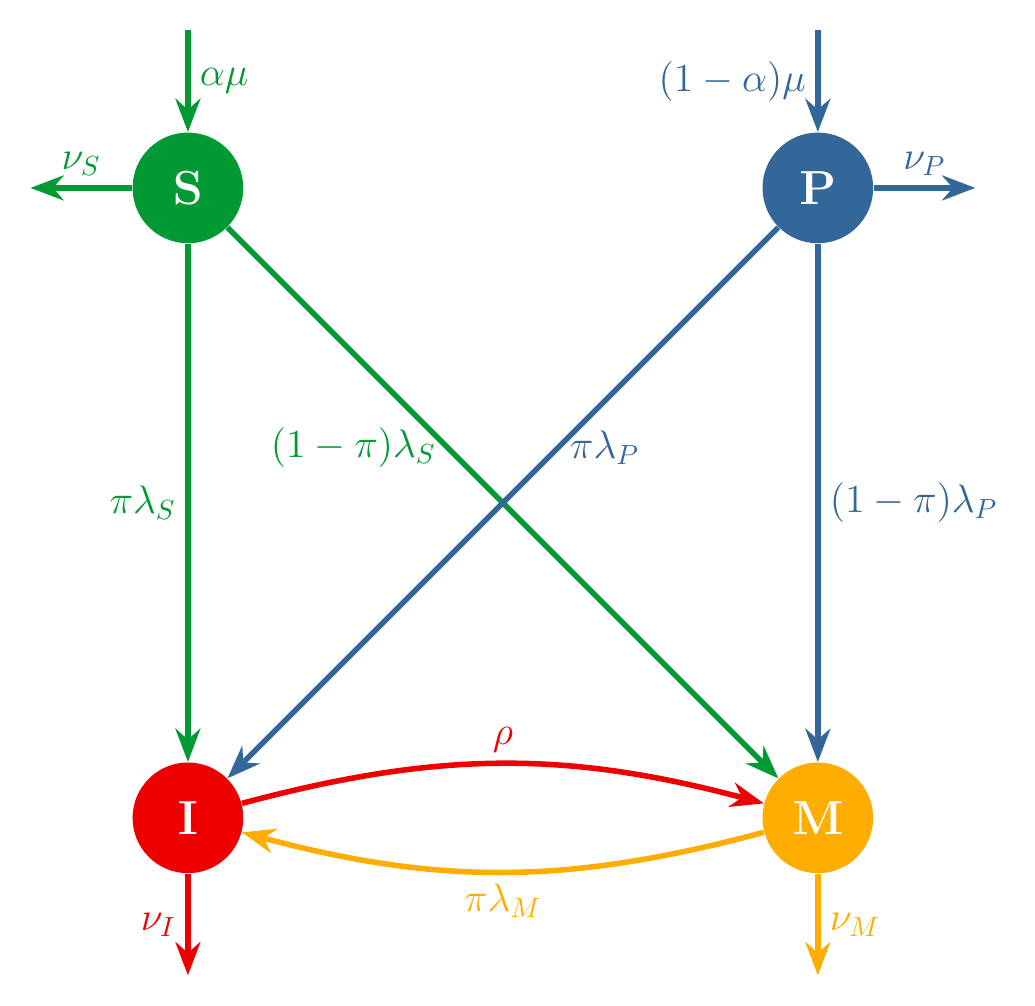
\begin{tikzpicture}
        \node[
            circle, 
            fill = ColorS,
            text = white,
            font = \bfseries\LARGE,
            minimum size = 40pt,
            inner sep = 0pt
        ] (S) at (0, 0) {S};
        \node[
            circle, 
            fill = ColorP,
            text = white,
            font = \bfseries\LARGE,
            minimum size = 40pt,
            inner sep = 0pt
        ] (P) at (8, 0) {P};
        \node[
            circle, 
            fill = ColorI,
            text = white,
            font = \bfseries\LARGE,
            minimum size = 40pt,
            inner sep = 0pt
        ] (I) at (0, -8) {I};
        \node[
            circle, 
            fill = ColorM,
            text = white,
            font = \bfseries\LARGE,
            minimum size = 40pt,
            inner sep = 0pt
        ] (M) at (8, -8) {M};

        \draw[
            -Stealth,
            draw = ColorS,
            line width = 2pt
        ] (S) -- node[left, font = \Large, text = ColorS] {$ \pi \lambda_S $} (I);
        \draw[
            -Stealth,
            draw = ColorS,
            line width = 2pt
        ] (S) -- node[left, pos = 0.4, font = \Large, text = ColorS] {$ (1-\pi) \lambda_S $} (M);
        \draw[
            -Stealth,
            draw = ColorP,
            line width = 2pt
        ] (P) -- node[right, pos = 0.4, font = \Large, text = ColorP] {$ \pi \lambda_P $} (I);
        \draw[
            -Stealth,
            draw = ColorP,
            line width = 2pt
        ] (P) -- node[right, font = \Large, text = ColorP] {$ (1-\pi) \lambda_P $} (M);

        \draw[
            -Stealth,
            draw = ColorI,
            line width = 2pt
        ] (I) to[bend left=15] node[above, font = \Large, text = ColorI] {$ \rho $} (M);
        \draw[
            -Stealth,
            draw = ColorM,
            line width = 2pt
        ] (M) to[bend left=15] node[below, font = \Large, text = ColorM] {$ \pi \lambda_M $} (I);

        \draw[
            Stealth-,
            draw = ColorS,
            line width = 2pt
        ] (S) -- node[right, font = \Large, text = ColorS] {$ \alpha \mu $} ++(90:2cm);
        \draw[
            -Stealth,
            draw = ColorS,
            line width = 2pt
        ] (S) -- node[above, font = \Large, text = ColorS] {$ \nu_S $} ++(180:2cm);
        \draw[
            Stealth-,
            draw = ColorP,
            line width = 2pt
        ] (P) -- node[left, font = \Large, text = ColorP] {$ (1-\alpha) \mu $} ++(90:2cm);
        \draw[
            -Stealth,
            draw = ColorP,
            line width = 2pt
        ] (P) -- node[above, font = \Large, text = ColorP] {$ \nu_P $} ++(0:2cm);
        \draw[
            -Stealth,
            draw = ColorI,
            line width = 2pt
        ] (I) -- node[left, font = \Large, text = ColorI] {$ \nu_I $} ++(270:2cm);
        \draw[
            -Stealth,
            draw = ColorM,
            line width = 2pt
        ] (M) -- node[right, font = \Large, text = ColorM] {$ \nu_M $} ++(270:2cm);
    \end{tikzpicture}
    \caption{Diagramma dei flussi}\label{fig:flussi}
\end{figure}

\subsection{Domini dei parametri e delle funzioni}\label{sec:domini}

In questa sezione vengono riportati i domini di tutti i parametri e le funzioni del modello. Per ciascuno indichiamo il simbolo, il dominio e un breve commento che ne spiega il ruolo e le limitazioni. I parametri che saranno specificati nelle funzioni di esempio non sono inclusi.

\begin{itemize}
    \item $\alpha \in [0, 1]$ \\
        Rappresenta la frazione di nuovi ingressi che è sana. La restante frazione $1-\alpha$ entra nella popolazione $P$. Il valore $\alpha = 0$ corrisponde al caso in cui tutti i nuovi ingressi hanno infortuni pregressi, mentre $\alpha = 1$ corrisponde al caso in cui tutti i nuovi ingressi sono sani.
    \item $\beta_S, \beta_P, \beta_I, \beta_M \in [0, 1]$ \\
        Sono i moltiplicatori di abbandono per ciascuna popolazione e modulano il tasso di abbandono nella funzione $\nu$. Se $\beta_\cdot = 0$ l'impatto dell'abbandono su quella popolazione è nullo, mentre se $\beta_\cdot = 1$ è massimo.
    \item $\gamma_S, \gamma_P, \gamma_M \in [0, 1]$ \\
        Sono i moltiplicatori di rischio nella funzione di infortunio e modulano la probabilità che un atleta si infortuni. Se $\gamma_\cdot = 0$ l'impatto dell'infortunio su quella popolazione è nullo, mentre se $\gamma_\cdot = 1$ è massimo. \\
        Si assume $\gamma_S \leq \gamma_P \leq \gamma_M$, a riflettere il fatto che gli atleti con infortuni pregressi o in corso sono considerati più a rischio rispetto agli atleti sani.
    \item $\pi \in [0, 1]$ \\
        Rappresenta la probabilità che un infortunio sia grave e porti l'atleta in $I$. La probabilità che sia lieve e porti l'atleta in $M$ è $1-\pi$. Il valore $\pi = 0$ corrisponde al caso in cui tutti gli infortuni sono lievi, mentre $\pi = 1$ corrisponde al caso in cui tutti gli infortuni sono gravi.
    \item $\rho \in [0, 1]$ \\
        Rappresenta il tasso di transizione da $I$ a $M$, cioè la frazione di atleti infortunati che, per unità di tempo, torna allenabile con qualche restrizione. Il valore $\rho = 0$ corrisponde a nessun recupero, mentre $\rho = 1$ corrisponde al caso in cui tutti gli infortunati tornano allenabili, passando in $M$, in un solo passo.
    \item $A_{\max} \in \mathbb{R}_{>0}$ \\
        Rappresenta la scala di riferimento per la densità sul tatami, cioè il numero massimo di atleti per cui l'allenamento è considerato sicuro. La densità può superare $1$, ma il rischio diventa molto alto. Il valore $A_{\max} = 1$ corrisponde al caso in cui un solo atleta satura il tatami, mentre valori più grandi corrispondono a tatami più capienti.
    \item $\mu : [0, 1] \longrightarrow \mathbb{R}_{\geq 0}$ \\
        È la funzione di crescita, non negativa, continua e limitata. Rappresenta il numero complessivo di nuovi ingressi alla frazione di tempo $\frac{t}{T}$ e riflette le dinamiche di iscrizione a una stagione sportiva. Si assume che $\mu$ sia approssimativamente decrescente, a riflettere il fatto che gli ingressi tendono a concentrarsi all'inizio del periodo.
    \item $\nu : {[0, 1]}^2 \longrightarrow [0, 1]$ \\
        È la funzione di abbandono, non negativa, continua e limitata. Rappresenta la frazione di atleti che abbandona il gruppo in ogni seduta, modulata dal parametro $\beta_\cdot$. Si assume che $\nu$ sia approssimativamente crescente, a riflettere il fatto che gli abbandoni tendono a concentrarsi alla fine del periodo.
    \item $\lambda : \mathbb{R}_{\geq 0}^3 \times [0, 1] \longrightarrow [0, 1]$ \\
        È la funzione di infortunio, non negativa, continua, limitata e crescente rispetto agli argomenti. Rappresenta la probabilità che un atleta si infortuni in una seduta e si satura a un valore massimo controllato da $\gamma_\cdot \in [0, 1]$, cioè $\lambda(\cdot, \cdot, \cdot, \gamma_\cdot) \leq \gamma_\cdot$. Il limite superiore $\lambda \leq \gamma_\cdot$ garantisce che la probabilità di infortunio non superi il moltiplicatore di rischio.
    \item $c_f, c_p : \{0, 1, \dots, T\} \longrightarrow \mathbb{R}_{\geq 0}$ \\
        Sono le funzioni di carico fisico e psicologico della seduta, non negative. Rappresentano la quantità di fatica aggiunta in ogni seduta e possono essere costanti, periodiche o variabili nel tempo. Non hanno limite superiore esplicito, ma nella pratica sono limitate dal carico massimo che un atleta può sostenere.
    \item $r : \{0, 1, \dots, T\} \longrightarrow [0, 1]$ \\
        È la funzione di recupero, non negativa e limitata. Rappresenta il tasso di smaltimento della fatica in ogni seduta. Il limite superiore $r \leq 1$ garantisce che la fatica non possa essere smaltita più di quanto sia stata accumulata.
\end{itemize}

\subsection{Vincoli di integrità}

In questa sottosezione vengono riportati i vincoli di integrità del modello. Per ciascuno indichiamo la formulazione, il ruolo e le condizioni che esso impone. I vincoli di integrità garantiscono che le variabili di stato rimangano non negative, che le uscite da ciascuna popolazione non superino il contenuto della popolazione stessa e che le transizioni tra popolazioni siano conservative. Essi costituiscono le condizioni minime affinché il modello sia ben posto e le sue soluzioni abbiano significato fisico. \par

Per ogni $t \in \{0, 1, \dots, T\}$ si deve avere che le popolazioni e le funzioni di fatica non diventino negative. Poiché le popolazioni evolvono secondo equazioni in cui compaiono tassi di uscita, la condizione di non negatività si traduce in un vincolo sul tasso di uscita complessivo da ciascuna popolazione. In particolare, il tasso di uscita non deve superare $1$, altrimenti la popolazione corrispondente diventerebbe negativa al passo successivo. I vincoli sono:
\begin{itemize}
    \item Vincolo per la non negatività di $S$:
        \[
            \nu\left(\frac{t}{T}, \beta_S\right) + \lambda\left(\bar{F}_f(t), \bar{F}_p(t), \frac{S(t) + P(t) + M(t)}{A_{\max}}, \gamma_S\right) \leq 1
        \]
    \item Vincolo per la non negatività di $P$:
        \[
            \nu\left(\frac{t}{T}, \beta_P\right) + \lambda\left(\bar{F}_f(t), \bar{F}_p(t), \frac{S(t) + P(t) + M(t)}{A_{\max}}, \gamma_P\right) \leq 1
        \]
    \item Vincolo per la non negatività di $I$:
        \[
            \rho + \nu\left(\frac{t}{T}, \beta_I\right) \leq 1
        \]
    \item Vincolo per la non negatività di $M$:
        \[
            \pi \lambda\left(\bar{F}_f(t), \bar{F}_p(t), \frac{S(t) + P(t) + M(t)}{A_{\max}}, \gamma_M\right) + \nu\left(\frac{t}{T}, \beta_M\right) \leq 1
        \]
    \item Vincolo per la non negatività di $\bar{F}_f$ e $\bar{F}_p$ (insieme a $c_f(t), c_p(t) \geq 0$):
        \[
            r(t) \leq 1
        \]
\end{itemize}
Poiché $\nu\left(\cdot, \beta_\cdot\right) \leq \beta_\cdot$ e $\lambda\left(\cdot, \cdot, \cdot, \gamma_\cdot\right) \leq \gamma_\cdot$, una condizione sufficiente, indipendente dallo stato del sistema, affinché i vincoli precedenti siano soddisfatti per ogni $t$ è
\[
    \beta_S + \gamma_S \leq 1, \qquad
    \beta_P + \gamma_P \leq 1, \qquad
    \rho + \beta_I \leq 1, \qquad
    \pi \gamma_M + \beta_M \leq 1.
\]

A questi vincoli si aggiunge il vincolo di conservazione della popolazione totale. Detta:
\[
    N(t) = S(t) + P(t) + I(t) + M(t)
\]
la popolazione totale al tempo $t$, si richiede che l'evoluzione di $N(t)$ sia descritta da:
\begin{align*}
    N(t+1) &= N(t) + \mu\left(\frac{t}{T}\right) \\
        &- \nu\left(\frac{t}{T}, \beta_S\right) S(t) \\
        &- \nu\left(\frac{t}{T}, \beta_P\right) P(t) \\
        &- \nu\left(\frac{t}{T}, \beta_I\right) I(t) \\
        &- \nu\left(\frac{t}{T}, \beta_M\right) M(t).
\end{align*}
Il vincolo garantisce che la popolazione totale cambi solo per effetto degli ingressi e degli abbandoni, e che le transizioni interne tra popolazioni siano conservative. Se il vincolo fosse violato, ci sarebbe una perdita o una creazione di atleti non giustificata dal modello. La conservazione è una conseguenza diretta della struttura delle equazioni delle popolazioni, in cui ogni transizione interna compare con segno opposto in due popolazioni diverse.
    \chapter{Le funzioni del modello}

Nel capitolo precedente abbiamo scritto le equazioni del modello e abbiamo introdotto le funzioni che vi compaiono: la funzione di crescita $\mu$, la funzione di abbandono $\nu$, la funzione di infortunio $\lambda$, le funzioni di carico $c_f$ e $c_p$ e la funzione di recupero $r$. In quel contesto ci siamo limitati a descriverne il ruolo e a specificarne i domini, senza scegliere una forma analitica. \\
In questo capitolo completiamo il modello, definendo per ogni funzione un esempio concreto di forma analitica, i parametri che la controllano, le proprietà che soddisfa e il significato dei suoi parametri. \par

La scelta della forma analitica non è mai neutra. Da un lato, la forma deve rispettare i domini, le limitazioni e le condizioni di coerenza discusse nel capitolo precedente. Dall'altro, deve essere abbastanza flessibile da rappresentare i fenomeni che vogliamo modellare, ma anche abbastanza semplice da permettere l'analisi e la simulazione. Tra questi due estremi esiste un compromesso, e la scelta dipende dagli obiettivi del modello e dai dati disponibili. In questo capitolo adottiamo un criterio esplicito: scegliamo forme analitiche continue, limitate, monotone dove serve e con parametri interpretabili, in modo che il modello resti trattabile e le sue conclusioni siano comprensibili. \par

La funzione di crescita, per esempio, deve riflettere il fatto che gli ingressi tendono a concentrarsi all'inizio del periodo e a ridursi nel tempo. La funzione di abbandono deve riflettere il fatto che gli abbandoni tendono a concentrarsi alla fine. La funzione di infortunio deve crescere con la fatica e con la densità, e saturare a un valore massimo. La funzione di recupero deve decrescere nel tempo, perché il recupero è più efficace all'inizio e più lento quando la fatica si accumula. Le funzioni di carico, infine, devono essere abbastanza flessibili da rappresentare scenari diversi, senza vincolare il modello a una forma specifica.

\section{Funzione di crescita}

La funzione di crescita $\mu$ descrive il numero complessivo di nuovi atleti che entrano nel gruppo in ogni seduta. Riflette la dinamica di iscrizione a una stagione sportiva e costituisce, insieme alla funzione di abbandono $\nu$, uno dei due flussi esterni del modello. \par

La forma analitica che adottiamo per la funzione di crescita è la seguente:
\[
    \mu(x) = \omega_\mu \exp\left(-\frac{x^2}{2 \sigma_\mu^2}\right)
\]
dove:
\begin{itemize}
    \item $x = \frac{t}{T} \in [0, 1]$ è la frazione di tempo trascorsa
    \item $\omega_\mu \in \mathbb{R}_{\geq 0}$ è l'ampiezza della funzione
    \item $\sigma_\mu \in \mathbb{R}_{> 0}$ è la larghezza del picco della funzione
\end{itemize}
La funzione è una gaussiana centrata in $x = 0$, troncata al dominio $[0, 1]$. Il massimo si trova in $x = 0$ ed è pari a $\omega_\mu$, mentre il valore in $x = 1$ è $\omega_\mu \exp\left(-\frac{1}{2 \sigma_\mu^2}\right)$. La funzione è non negativa, continua, derivabile e decrescente su tutto il dominio. \par

La scelta della gaussiana è motivata da tre ragioni. In primo luogo, è una funzione semplice e ben nota, con parametri interpretabili e proprietà analitiche note. In secondo luogo, centrata in $x = 0$ riflette il fatto che gli ingressi tendono a concentrarsi all'inizio del periodo, quando l'entusiasmo e la disponibilità sono maggiori, e a ridursi progressivamente nel tempo. In terzo luogo, ha una forma regolare e derivabile, che facilita l'analisi del modello e la derivazione di proprietà qualitative.

\begin{figure}[ht]
    \centering
    \includegraphics[width = \textwidth]{functions/mu.pdf}
    \caption{Funzione generica di crescita $\mu$}
\end{figure}

\subsection{Parametri}

La funzione di crescita dipende da due parametri, $\omega_\mu$ e $\sigma_\mu$, che hanno domini e significati distinti. \par

Il parametro $\omega_\mu \in \mathbb{R}_{\geq 0}$ rappresenta l'ampiezza massima della funzione di crescita, cioè il numero massimo di nuovi atleti che entrano nel gruppo in una singola seduta. Il valore $\omega_\mu = 0$ corrisponde al caso in cui non ci sono nuovi ingressi, mentre valori più grandi corrispondono a ingressi più numerosi. \\
Nella pratica, $\omega_\mu$ è limitato dal numero massimo di atleti che la palestra può accogliere e dal bacino di utenza disponibile. Il parametro $\omega_\mu$ ha come unità di misura il numero di atleti. Un valore grande di $\omega_\mu$ corrisponde a una palestra capace di accogliere molti nuovi atleti, mentre un valore piccolo corrisponde a una palestra con capacità limitata. Il parametro $\omega_\mu$ può essere stimato dai dati storici di iscrizione, oppure scelto in base a scenari ipotetici.

Il parametro $\sigma_\mu \in \mathbb{R}_{> 0}$ rappresenta la larghezza del picco della funzione di crescita, cioè la velocità con cui gli ingressi decadono nel tempo. Valori piccoli di $\sigma_\mu$ corrispondono a un picco stretto, cioè a ingressi concentrati nelle prime sedute e rapidamente decrescenti. Valori grandi di $\sigma_\mu$ corrispondono a un picco largo, cioè a ingressi distribuiti su un periodo più lungo. \\
Un valore piccolo di $\sigma_\mu$, come mostrato in \autoref{fig:function-mu-sigma}, corrisponde a una stagione in cui gli ingressi si concentrano nelle prime settimane e poi si esauriscono, mentre un valore grande corrisponde a una stagione in cui gli ingressi sono distribuiti su un periodo più lungo.

\begin{figure}[ht]
    \centering
    \includegraphics[width = \textwidth]{functions/mu_sigma.pdf}
    \caption{Funzione di crescita $\mu$ al variare del parametro $\sigma_\mu$}\label{fig:function-mu-sigma}
\end{figure}

\subsection{Proprietà}\label{sec:function-mu-property}

La funzione di crescita soddisfa le seguenti proprietà, che discendono direttamente dalla sua forma analitica e dai domini dei parametri. \par

La funzione è non negativa, cioè $\mu(x) \geq 0$ per ogni $x \in [0, 1]$. Questa proprietà è garantita dal fatto che l'esponenziale è sempre positivo e $\omega_\mu \geq 0$.

La funzione è continua e derivabile su tutto il dominio, per definizione. La derivata prima è
\[
    \frac{d}{dx} \mu(x) = -\omega_\mu \frac{x}{\sigma_\mu^2} \exp\left(-\frac{x^2}{2 \sigma_\mu^2}\right)
\]
che è negativa per $x > 0$. Quindi la funzione è monotona decrescente su $[0, 1]$, con un massimo in $x = 0$.

Il valore massimo è:
\[
    \max_{x \in [0, 1]} \mu(x) = \mu(0) = \omega_\mu,
\]
mentre il valore minimo sul dominio è:
\[
    \min_{x \in [0, 1]} \mu(x) = \mu(1) = \omega_\mu \exp\left(-\frac{1}{2 \sigma_\mu^2}\right).
\]
Il rapporto tra $\mu(1)$ e $\mu(0)$ è:
\[
    \frac{\mu(1)}{\mu(0)} = \exp\left(-\frac{1}{2 \sigma_\mu^2}\right)
\]
che dipende solo da $\sigma_\mu$. Per $\sigma_\mu$ piccolo, il rapporto è prossimo a zero, il che significa che gli ingressi si esauriscono rapidamente. Per $\sigma_\mu$ grande, il rapporto è prossimo a uno, il che significa che gli ingressi restano circa costanti. \par

La funzione è limitata superiormente da $\omega_\mu$ e inferiormente da zero; più precisamente, essendo continua e decrescente, la sua immagine è $\left[\omega_\mu \exp\left(-\frac{1}{2 \sigma_\mu^2}\right), \omega_\mu\right] \subseteq [0, \omega_\mu]$. Questa proprietà garantisce che il numero di nuovi ingressi non superi mai l'ampiezza massima $\omega_\mu$, coerentemente con il significato del parametro.

\section{Funzione di abbandono}

La funzione di abbandono $\nu$ descrive la frazione di atleti che abbandona il gruppo in ogni seduta. Costituisce, insieme alla funzione di crescita $\mu$, uno dei due flussi esterni del modello, e regola la diminuzione della popolazione. \par

La forma analitica che adottiamo per la funzione di abbandono è la seguente:
\[
    \nu(x, \beta) = \beta \exp\left(-\frac{(x - 1)^2}{2 \sigma_\nu^2}\right)
\]
dove:
\begin{itemize}
    \item $x = \frac{t}{T} \in [0, 1]$ è la frazione di tempo trascorsa
    \item $\beta \in [0, 1]$ è l'ampiezza della funzione
    \item $\sigma_\nu \in \mathbb{R}_{> 0}$ è la larghezza del picco della funzione
\end{itemize}
La funzione è una gaussiana centrata in $x = 1$, troncata al dominio $[0, 1]$. Il massimo si trova in $x = 1$ ed è pari a $\beta$, mentre il valore in $x = 0$ è $\beta \exp\left(-\frac{1}{2 \sigma_\nu^2}\right)$. \par

A meno dell'ampiezza e della larghezza, la funzione è la riflessione della funzione $\mu$ rispetto alla retta $x = \frac{1}{2}$: infatti, se $\beta = \omega_\mu$ e $\sigma_\nu = \sigma_\mu$, si ha $\nu(x, \beta) = \mu(1 - x)$. Mentre gli ingressi tendono a concentrarsi all'inizio del periodo, gli abbandoni tendono a concentrarsi alla fine, quando l'entusiasmo iniziale si riduce, sopraggiungono altri impegni o la stanchezza accumulata diventa significativa. La simmetria tra le due funzioni non è casuale, ma riflette il fatto che i due fenomeni hanno dinamiche temporali opposte. La scelta della gaussiana permette di rappresentare questa opposizione con una forma semplice e ben nota, con parametri interpretabili e proprietà analitiche note. \par

La funzione $\nu$ dipende anche dal moltiplicatore $\beta$, passato come argomento, che permette di differenziare il tasso di abbandono tra le diverse popolazioni. Nel modello, $\beta$ assume valori diversi a seconda della popolazione a cui la funzione si applica: $\beta_S$ per i sani, $\beta_P$ per i pregressi, $\beta_I$ per gli infortunati e $\beta_M$ per i malconci. Questa scelta riflette il fatto che gli atleti in popolazioni diverse possono avere comportamenti di abbandono diversi, a causa della loro condizione fisica, della loro motivazione o del loro rapporto con l'attività. \par

Le proprietà della funzione $\nu$ sono le stesse della funzione $\mu$ descritte in \autoref{sec:function-mu-property}, con la sostituzione di $\omega_\mu$ con $\beta$ e di $\sigma_\mu$ con $\sigma_\nu$, e con la differenza che la funzione è crescente anziché decrescente.

\begin{figure}[ht]
    \centering
    \includegraphics[width = \textwidth]{functions/nu.pdf}
    \caption{Funzione generica di abbandono $\nu$}
\end{figure}

\subsection{Parametri}

La funzione di abbandono dipende da due parametri, $\beta$ e $\sigma_\nu$, che hanno domini e significati distinti. \par

Il parametro $\beta \in [0, 1]$ rappresenta l'ampiezza massima della funzione di abbandono, cioè la frazione massima di atleti che possono abbandonare in una singola seduta. Il valore $\beta = 0$ corrisponde al caso in cui non ci sono abbandoni dalla popolazione considerata, mentre $\beta = 1$ corrisponde al caso in cui il tasso di abbandono raggiunge il valore massimo consentito, cioè $1$. Nella pratica, $\beta$ è limitato dal fatto che il tasso di abbandono non può superare l'unità, altrimenti la popolazione diventerebbe negativa. Il parametro $\beta$ è adimensionale, perché rappresenta una frazione. \par

Il parametro $\sigma_\nu \in \mathbb{R}_{> 0}$, come per $\mu$, rappresenta la larghezza del picco della funzione di abbandono, cioè la velocità con cui gli abbandoni crescono nel tempo.

\section{Funzione di infortunio}

La funzione di infortunio $\lambda$ descrive la probabilità che un atleta si infortuni durante una seduta. È la funzione più importante del modello, perché collega la fatica e la densità sul tatami alla dinamica degli infortuni e, di conseguenza, alla composizione del gruppo. \par

La forma analitica che adottiamo per la funzione di infortunio è la seguente:
\[
    \lambda(f_f, f_p, d, \gamma) = \gamma \frac{1}{1 + \exp\left(-\omega_f f_f - \omega_p f_p - \omega_d d + b\right)},
\]
dove:
\begin{itemize}
    \item $f_f \in \mathbb{R}_{\geq 0}$ è la fatica fisica
    \item $f_p \in \mathbb{R}_{\geq 0}$ è la fatica psicologica
    \item $d \in \mathbb{R}_{\geq 0}$ è la densità di atleti
    \item $\gamma \in [0, 1]$ è l'ampiezza della funzione
    \item $\omega_f, \omega_p, \omega_d \in \mathbb{R}_{> 0}$ sono pesi positivi
    \item $b \in \mathbb{R}_{\geq 0}$ è un fattore di soglia
\end{itemize}
Il suo valore è compreso tra $0$ e $\gamma$, ed è crescente rispetto a $f_f$, $f_p$ e $d$. \par

La scelta della sigmoide è motivata da tre ragioni. In primo luogo, è una funzione limitata, con valori compresi tra $0$ e $1$, il che garantisce che la probabilità di infortunio non superi mai il moltiplicatore $\gamma$. In secondo luogo, è crescente e saturante, il che riflette il fatto che il rischio di infortunio cresce con la fatica e la densità, ma non può crescere all'infinito. In terzo luogo, è regolare e derivabile, il che facilita l'analisi del modello. Il fattore di soglia $b$ sposta la sigmoide verso destra, riducendo il rischio in assenza di fatica e densità.

\begin{figure}[ht]
    \centering
    \includegraphics[width = \textwidth]{functions/lambda_ff.pdf}
    \caption{Funzione di infortunio $\lambda$ al variare del parametro $f_f$}
\end{figure}

\subsection{Parametri}

La funzione di infortunio dipende da cinque parametri, $\gamma$, $\omega_f$, $\omega_p$, $\omega_d$ e $b$, che hanno domini e significati distinti. \par

Il parametro $\gamma \in [0,1]$, analogo di $\beta$ per $\nu$, rappresenta il moltiplicatore di rischio specifico della popolazione a cui la funzione si applica. Il valore $\gamma = 0$ corrisponde al caso in cui la popolazione non ha rischio di infortunio, mentre $\gamma = 1$ corrisponde al caso in cui il rischio massimo è pari a $1$. Nel modello, $\gamma$ assume valori diversi a seconda della popolazione: $\gamma_S$ per i sani, $\gamma_P$ per i pregressi e $\gamma_M$ per i malconci. Si assume $\gamma_S \leq \gamma_P \leq \gamma_M$, a riflettere il fatto che gli atleti con infortuni pregressi o in corso sono considerati più a rischio rispetto agli atleti sani. \par

I parametri $\omega_f, \omega_p, \omega_d \in \mathbb{R}_{> 0}$ rappresentano il peso rispettivamente della fatica fisica, della fatica psicologica e della densità di atleti sul tatami. Il valore $\omega_\cdot \to 0^+$ corrisponde al caso in cui la variabile non influenza il rischio, mentre valori più grandi corrispondono a una dipendenza più forte. \par

Il parametro $b \in \mathbb{R}_{\geq 0}$ rappresenta il fattore di traslazione del valore di soglia. Il ruolo di $b$ è quello di evitare che un atleta fresco in un tatami vuoto abbia un rischio di infortunio non trascurabile. Senza $b$, il rischio in assenza di fatica e densità sarebbe $\frac{\gamma}{2}$, che potrebbe essere troppo alto.

\subsection{Proprietà}

La funzione di infortunio soddisfa le seguenti proprietà, che derivano direttamente dalla sua forma analitica e dai domini dei parametri. \par

La funzione è non negativa, cioè $\lambda(f_f, f_p, d, \gamma) \geq 0$ per ogni valore degli argomenti. Questa proprietà è garantita dal fatto che la sigmoide è sempre positiva e $\gamma \geq 0$. \par

La funzione è limitata superiormente da $\gamma$, cioè $\lambda(f_f, f_p, d, \gamma) \leq \gamma$. Questa proprietà è garantita dal fatto che la sigmoide è limitata superiormente da $1$ e $\gamma \in [0, 1]$. Il limite superiore $\lambda \leq \gamma$ garantisce che la probabilità di infortunio non superi mai $1$. \par

La funzione è continua e derivabile su tutto il dominio, per definizione. Le derivate parziali rispetto a $f_f$, $f_p$ e $d$ sono positive, perché la sigmoide è crescente rispetto al suo argomento. Quindi la funzione è monotona crescente rispetto a $f_f$, $f_p$ e $d$. \par

La funzione è lineare rispetto a $\gamma$, cioè $\lambda(f_f, f_p, d, \gamma) = \gamma \cdot s\left(\omega_f f_f + \omega_p f_p + \omega_d d - b\right)$, dove $s(z) = \frac{1}{1 + e^{-z}}$ è la sigmoide logistica. Questa proprietà permette di separare il contributo del moltiplicatore di rischio da quello della fatica e della densità. \par

Il valore in assenza di fatica e densità è $\lambda(0, 0, 0, \gamma) = \frac{\gamma}{1 + e^b}$. Per $b = 0$, questo valore è $\frac{\gamma}{2}$, mentre per $b$ grande, questo valore tende a zero. La scelta di $b$ controlla quindi il rischio di base in assenza di fatica e densità. \par

Il limite per $f_f, f_p, d \to +\infty$ è $\lambda \to \gamma$, cioè la funzione satura al valore massimo consentito. Questo riflette il fatto che, per fatica e densità molto elevate, il rischio di infortunio raggiunge il suo massimo e non può crescere ulteriormente.

\section{Funzioni di carico}

Le funzioni di carico $c_f$ e $c_p$ descrivono la quantità di fatica fisica e psicologica aggiunta in ogni seduta di allenamento. Costituiscono l'ingresso principale del modello per la dinamica della fatica e sono trattate come parametri esogeni. In questa sezione non adottiamo una forma analitica specifica, ma presentiamo tre esempi che illustrano come il carico possa essere costante, periodico o variabile. La scelta tra questi esempi dipende dal fenomeno modellato e dai dati disponibili, e il modello è progettato per accogliere qualsiasi funzione che rispetti i domini e i vincoli discussi nel capitolo precedente.

\paragraph{Carico costante}
Il primo esempio è il carico costante, in cui le funzioni di carico assumono lo stesso valore in ogni seduta. Formalmente, si ha:
\begin{gather*}
    c_f(t) = c_{f, 0} \in \mathbb{R}_{\geq 0} \\
    c_p(t) = c_{p, 0} \in \mathbb{R}_{\geq 0}
\end{gather*}
dove $c_{f,0}$ e $c_{p,0}$ sono costanti non negative. Questo esempio, come rappresentato in \autoref{fig:function-c-costante}, corrisponde a un programma di allenamento uniforme, in cui ogni seduta ha lo stesso carico fisico e psicologico. È il caso più semplice e permette di studiare il comportamento del modello in condizioni stazionarie, senza l'effetto della stagionalità. Nella pratica, il carico costante è raramente realistico per un'intera stagione, ma può essere una buona approssimazione per periodi brevi o per studiare l'effetto della fatica in condizioni controllate.

\begin{figure}[ht]
    \centering
    \includegraphics[width = \textwidth]{functions/c_costante.pdf}
    \caption{Funzione di carico costante}\label{fig:function-c-costante}
\end{figure}

\paragraph{Carico periodico}
Il secondo esempio è il carico periodico, in cui le funzioni di carico oscillano con una periodicità legata, ad esempio, al microciclo di allenamento. Come rappresentato in \autoref{fig:function-c-periodico}, consideriamo il caso in cui in ogni periodo di tre sedute si alternano un allenamento ad alto carico (ad esempio randori), un allenamento a carico medio (ad esempio tecnica) e un allenamento senza carico (ad esempio riposo o seduta di allungamento). Formalmente, per $n \in \mathbb{N}$, si ha
\[
    c_f(t) = c_p(t) = \begin{cases}
        1 & \text{se } t = 3n, \\
        0.5 & \text{se } t = 3n + 1, \\
        0 & \text{se } t = 3n + 2.
    \end{cases}
\]
Questa forma può essere scritta in modo compatto come
\[
    c_f(t) = c_p(t) = \frac{1}{2}\left((2 - t) \bmod 3\right),
\]
dove l'operatore $\bmod$ restituisce il resto della divisione intera. La funzione è periodica con periodo $3$ e rappresenta un ciclo di allenamento in cui il carico varia tra alto, medio e nullo. La scelta di questa forma è motivata dalla necessità di rappresentare la periodicità del carico su scale temporali brevi, senza introdurre una forma analitica continua. Il carico periodico è una funzione definita su un dominio discreto e rispetta i vincoli di integrità del modello, perché i suoi valori sono non negativi. Affinché la fatica resti inoltre limitata nel tempo, il tasso di recupero deve essere sufficientemente grande da smaltire la fatica accumulata.

\begin{figure}[ht]
    \centering
    \includegraphics[width = \textwidth]{functions/c_periodico.pdf}
    \caption{Funzione di carico periodico}\label{fig:function-c-periodico}
\end{figure}

\paragraph{Carico variabile}
Il terzo esempio è il carico variabile, in cui le funzioni di carico sono assegnate in modo arbitrario, seduta per seduta. Formalmente, si può scrivere:
\begin{gather*}
    c_f \colon \{0, 1, \dots, T\} \to \mathbb{R}_{\geq 0} \\
    c_p \colon \{0, 1, \dots, T\} \to \mathbb{R}_{\geq 0}
\end{gather*}
Questo esempio corrisponde a un programma di allenamento dettagliato, in cui ogni seduta ha un carico specifico, eventualmente diverso dalle altre. Il carico variabile è il caso più generale e permette di rappresentare scenari arbitrari, come periodi di allenamento intenso seguiti da periodi di recupero, sedute di tecnica alternate con sedute di randori, o variazioni improvvise del carico dovute a eventi esterni. \\
La forma variabile, come rappresentato in \autoref{fig:function-c-variabile}, non richiede una forma analitica specifica, ma solo che le funzioni siano non negative e limitate. Il carico variabile rispetta i vincoli di integrità del modello a patto che i suoi valori siano non negativi; come nel caso periodico, affinché la fatica resti limitata il tasso di recupero deve essere sufficientemente grande da smaltire la fatica accumulata.

\begin{figure}[ht]
    \centering
    \includegraphics[width = \textwidth]{functions/c_variabile.pdf}
    \caption{Funzione di carico variabile}\label{fig:function-c-variabile}
\end{figure}

\section{Funzione di recupero}

La funzione di recupero $r$ descrive il tasso di smaltimento della fatica in ogni seduta. Regola la dinamica della fatica e costituisce, insieme alle funzioni di carico, uno dei due termini che determinano l'evoluzione di $\bar{F}_f$ e $\bar{F}_p$. \par

La forma analitica che adottiamo per la funzione di recupero è la seguente:
\[
    r(t) = 2 \omega_r \frac{1}{1 + \exp\left(\sigma_r t\right)}
\]
dove:
\begin{itemize}
    \item $t \in \{0, 1, \dots, T\}$ è il tempo
    \item $\omega_r \in [0, 1]$ è l'ampiezza massima
    \item $\sigma_r \in \mathbb{R}_{\geq 0}$ è la velocità di decadimento
\end{itemize}
La funzione è una sigmoide decrescente, che parte da $\omega_r$ in $t = 0$ e tende a zero per $t \to +\infty$. La scelta della sigmoide decrescente è motivata dalla necessità di rappresentare il fatto che il recupero è massimo all'inizio del periodo, quando gli atleti sono freschi, e decresce nel tempo, man mano che la fatica si accumula. \par

La forma sigmoide permette di rappresentare scenari diversi variando i parametri. Se $\sigma_r = 0$, la funzione è costante e pari a $\omega_r$. Se $\sigma_r$ è grande, la funzione decade rapidamente verso zero. La sigmoide decrescente è una scelta naturale per rappresentare un recupero che si riduce nel tempo, e ha il vantaggio di essere limitata e derivabile.

\begin{figure}[ht]
    \centering
    \includegraphics[width = \textwidth]{functions/r.pdf}
    \caption{Funzione generica di recupero $r$}
\end{figure}

\subsection{Parametri}

Il parametro $\omega_r \in [0, 1]$ rappresenta l'ampiezza massima della funzione di recupero, cioè il tasso di recupero massimo che può essere raggiunto. Il valore $\omega_r = 0$ corrisponde al caso in cui non c'è recupero, mentre $\omega_r = 1$ corrisponde al caso in cui il recupero massimo è pari a $1$. Il limite superiore $\omega_r \leq 1$ garantisce che la fatica non diventi negativa, perché il termine di recupero $r(t) \bar{F}_\cdot(t)$ non supera $\bar{F}_\cdot(t)$. \par

Il parametro $\sigma_r \in \mathbb{R}_{\geq 0}$ rappresenta la velocità di decadimento del recupero. Il valore $\sigma_r = 0$ corrisponde a un recupero costante, mentre valori più grandi corrispondono a un recupero che decresce più rapidamente. Il parametro $\sigma_r$ controlla la scala temporale del decadimento, cioè quanto rapidamente il recupero passa da un valore alto a un valore basso.

\subsection{Proprietà}

La funzione di recupero soddisfa le seguenti proprietà, che derivano direttamente dalla sua forma analitica e dai domini dei parametri. \par

La funzione è non negativa, cioè $r(t) \geq 0$ per ogni $t$. Questa proprietà è garantita dal fatto che la sigmoide è sempre positiva e $\omega_r \geq 0$. \par

La funzione è limitata: il valore massimo è $r(0) = \omega_r$, mentre per $\sigma_r > 0$ il valore asintotico per $t \to +\infty$ è zero, che è l'estremo inferiore ma non viene mai raggiunto. Quindi l'immagine della funzione è contenuta in $(0, \omega_r] \subseteq [0, 1]$, compatibilmente con il vincolo $r(t) \leq 1$ richiesto per un tasso di recupero. \par

La funzione è continua e derivabile su tutto il dominio, per definizione. La derivata prima è
\[
    \frac{d}{dt} r(t) = -2 \omega_r \sigma_r \frac{\exp\left(\sigma_r t\right)}{\left(1 + \exp\left(\sigma_r t\right)\right)^2}
\]
che è negativa per ogni $t$ se $\sigma_r > 0$. Quindi la funzione è monotona decrescente.
    \chapter{Calibrazione dei parametri e simulazione}\label{chap:simulazione}

Nei capitoli precedenti abbiamo costruito il modello e scelto una forma analitica per ciascuna delle sue funzioni. Per poterlo simulare, tuttavia, è necessario assegnare un valore a tutti i parametri. In questo capitolo scegliamo tali valori e descriviamo la dinamica che ne deriva. \par

Non disponendo di dati reali con cui confrontare il modello, procediamo nel modo seguente: fissiamo alcuni requisiti che la dinamica deve rispettare, ad esempio quanto può calare il gruppo o quanti atleti possono essere infortunati, e cerchiamo i valori dei parametri che li soddisfano. In altre parole, invece di domandarci quali siano i valori ``veri'' dei parametri, che non possiamo conoscere senza dati, ci chiediamo quali valori producano un comportamento del gruppo coerente con quello che vogliamo rappresentare. \par

Lo scenario che costruiamo è sfavorevole, ma non estremo: rappresenta un periodo di allenamento intenso senza alcuna forma di prevenzione, con molti infortuni, in cui però il gruppo resta in gran parte unito e gli atleti sani raramente abbandonano. Nel capitolo successivo verrà introdotto un controllo, cioè le strategie di prevenzione a disposizione dell'allenatore, e questo scenario servirà come termine di confronto per misurarne l'efficacia. Se lo scenario di partenza presentasse pochi infortuni, il controllo avrebbe poco margine per migliorarlo e sarebbe difficile confrontare strategie diverse. Per questo motivo preferiamo partire da una situazione in cui gli infortuni sono un problema evidente.

\section{Impostazione della simulazione}

Fissiamo un orizzonte di $T = 50$ sedute di allenamento. Ipotizzando una seduta al giorno, tale orizzonte equivale a circa sette settimane, vale a dire un periodo di preparazione di durata media, paragonabile alla preparazione per una gara importante oppure a un raduno collegiale. La durata scelta è sufficientemente ampia da permettere di osservare l'accumulo della fatica e degli infortuni, ma al tempo stesso abbastanza contenuta da rispettare l'ipotesi secondo cui gli atleti infortunati non hanno il tempo di guarire del tutto. \par

Le condizioni iniziali sono:
\begin{gather*}
    S(0) = 400 \\
    P(0) = 100 \\
    I(0) = M(0) = 0 \\
    \bar{F}_f(0) = \bar{F}_p(0) = 0
\end{gather*}
Il gruppo di partenza è dunque formato da $N(0) = 500$ atleti, dei quali l'$80\%$ sani e il $20\%$ con infortuni pregressi. Inizialmente nessun atleta risulta infortunato e il gruppo è riposato, poiché assumiamo che il periodo cominci dopo una fase di recupero. La numerosità del gruppo è tale da consentire di trattare le popolazioni come numeri reali, come richiesto dalle ipotesi del modello. \par

La capienza del tatami è $A_{\max} = 800$ atleti. All'inizio del periodo la densità sul tatami è quindi pari a $0.625$: il tatami è affollato, ma non saturo. Nel corso del periodo la densità cala, poiché una parte degli atleti riporta infortuni gravi e smette di allenarsi e, nelle ultime settimane, alcuni abbandonano: alla fine essa scende a circa $0.48$.

\subsection{Carico di allenamento}

Il carico di allenamento costituisce una scelta dell'allenatore e non viene calibrato. Adottiamo il carico periodico presentato nel capitolo sulle funzioni, nel quale si susseguono una seduta ad alto carico, una a carico medio e una priva di carico:
\[
    c_f(t) = c_p(t) = \begin{cases}
        1 & \text{se } t = 3n \\
        0.5 & \text{se } t = 3n + 1 \\
        0 & \text{se } t = 3n + 2
    \end{cases}
\]
Tale carico corrisponde a un ciclo di tre giorni assai diffuso nella pratica: un giorno di randori intenso, un giorno di tecnica e una seduta leggera, di scarico, con esercizi a basso impegno come le cadute o lo stretching. Il carico medio per seduta risulta pari a $0.5$. \par

\begin{figure}[ht]
    \centering
    \includegraphics[width = 0.5\textwidth]{pictures/grip2.jpg}
    \caption[Esercizio a coppie]{Due judoka si preparano a un esercizio a coppie durante una seduta di tecnica, in cui il carico è intermedio.}
\end{figure}

Dato che carico fisico e carico psicologico coincidono, anche le due componenti della fatica sono uguali per ogni $t$, ovvero $\bar{F}_f(t) = \bar{F}_p(t)$. Questa scelta rende più semplice la lettura dei risultati e non compromette gli scopi del capitolo. La distinzione tra le due componenti assumerà rilevanza nel momento in cui si metteranno a confronto programmi di allenamento caratterizzati da un diverso equilibrio tra impegno fisico e impegno mentale. \par

È opportuno osservare che i parametri individuati valgono per questo specifico carico. Qualora l'allenatore modificasse il programma, i parametri del gruppo rimarrebbero invariati, ma la dinamica cambierebbe: proprio questo consentirà, in seguito, di confrontare programmi di allenamento differenti.

\section{Parametri delle funzioni}

I parametri si articolano in due gruppi. Il primo comprende i parametri delle funzioni $\mu$, $\nu$, $\lambda$ e $r$, che ne definiscono la forma. Il secondo comprende i parametri delle equazioni del modello, ovvero $\alpha$, $\pi$, $\rho$, i moltiplicatori di abbandono $\beta_\cdot$ e i moltiplicatori di rischio $\gamma_\cdot$. \par

I due gruppi svolgono un ruolo differente. I parametri delle funzioni descrivono \emph{in che modo} variano nel tempo ingressi, abbandoni, rischio e recupero. I parametri del modello descrivono invece \emph{quanto} tali fenomeni incidono su ciascuna popolazione. Per tale ragione li trattiamo separatamente: i parametri delle funzioni vengono fissati direttamente, in funzione del comportamento che intendiamo ottenere, mentre i parametri del modello sono calcolati nella sezione seguente. La separazione dei due gruppi consente inoltre di ridurre il numero di parametri da calcolare, da diciannove a dieci. \par

I valori scelti per i parametri delle funzioni sono riportati nella \autoref{tab:sim-funzioni} e commentati qui di seguito.

\begin{table}[ht]
    \centering
    \caption{Parametri delle funzioni del modello}\label{tab:sim-funzioni}
    \begin{tblr}{
        colspec = {cccl},
        hline{4,5,9} = {0.03em},
    }
        Funzione & Parametro & Valore & Significato \\
        \SetCell[r=2]{c} $\mu$ & $\omega_\mu$ & $5$ & ingressi nella prima seduta \\
              & $\sigma_\mu$ & $0.15$ & durata del periodo di ingresso \\
        $\nu$ & $\sigma_\nu$ & $0.15$ & durata del periodo di abbandono \\
        \SetCell[r=4]{c}$\lambda$ & $\omega_f$ & $0.5$ & peso della fatica fisica \\
                  & $\omega_p$ & $0.3$ & peso della fatica psicologica \\
                  & $\omega_d$ & $0.2$ & peso della densità \\
                  & $b$ & $1$ & soglia \\
        \SetCell[r=2]{c}$r$ & $\omega_r$ & $1$ & recupero iniziale \\
            & $\sigma_r$ & $0.05$ & velocità di decadimento del recupero \\
    \end{tblr}
\end{table}

\paragraph{Funzione di crescita}

Nel corso della prima seduta entrano $5$ nuovi atleti, dopodiché gli ingressi calano rapidamente. Complessivamente entrano circa $49$ nuovi atleti, ovvero circa il $10\%$ del gruppo iniziale, e quasi tutti, all'incirca $47$, arrivano entro le prime $15$ sedute. Superata la metà del periodo gli ingressi risultano praticamente nulli. \par

Tale profilo descrive un gruppo che si completa nelle prime due settimane: alcuni atleti giungono in ritardo, ad esempio per ragioni di lavoro, di studio o di trasporto, ma dopo questa fase il gruppo rimane chiuso. La crescita della popolazione nella fase iniziale del periodo dipende quasi esclusivamente da questi due parametri, poiché nelle prime settimane gli abbandoni sono trascurabili.

\paragraph{Funzione di abbandono}

Gli abbandoni presentano un andamento opposto. Il rapporto tra la funzione di abbandono e il suo valore massimo è praticamente nullo a metà del periodo, assume valore circa $0.08$ dopo due terzi del periodo, circa $0.41$ all'$80\%$ e circa $0.80$ al $90\%$, fino a raggiungere il massimo nell'ultima seduta. Gli abbandoni si concentrano dunque nelle ultime due settimane. \par

Ciò rispecchia quanto spesso si verifica nella pratica: verso la conclusione di un periodo di allenamento prolungato crescono gli impegni esterni, la stanchezza accumulata si fa sentire e alcuni atleti scelgono di interrompere anzitempo. L'entità con cui la funzione incide su ciascuna popolazione dipende dai moltiplicatori $\beta_\cdot$, calcolati nella sezione successiva.

\paragraph{Funzione di infortunio}

Il fattore di rischio più rilevante è la fatica fisica, seguita dalla fatica psicologica e dalla densità sul tatami. I pesi $\omega_f$, $\omega_p$ e $\omega_d$ rispecchiano esattamente questo ordine. La soglia $b = 1$ garantisce che, con il gruppo riposato, il rischio sia contenuto ma non nullo. \par

Per valutare l'entità del rischio è utile considerare il rapporto $\frac{\lambda}{\gamma_\cdot}$, che denominiamo rischio relativo: esso indica la frazione del rischio massimo $\gamma_\cdot$ effettivamente raggiunta ed è identico per tutte le popolazioni. Nella simulazione il rischio relativo cresce parallelamente alla fatica, passando da circa $0.29$ all'inizio a circa $0.79$ al termine del periodo. \par

Il rischio relativo si mantiene pertanto distante sia da zero sia dal suo valore massimo, pari a $1$. Ciò è rilevante: in questa fascia il rischio risulta sensibile alle variazioni della fatica, e dunque una modifica del carico di allenamento si traduce in una variazione effettiva del numero di infortuni.

\paragraph{Funzione di recupero}

La scelta più significativa concerne la velocità $\sigma_r$ con cui il recupero diminuisce. Nel capitolo sulle funzioni avevamo impiegato, a titolo di esempio, $\sigma_r = 0.2$. Con tale valore, tuttavia, il recupero si riduce quasi a zero già a metà del periodo: gli atleti non sono più in grado di smaltire la fatica, che cresce ininterrottamente fino a circa $18$. Dopo circa $25$ sedute il rischio relativo raggiunge $0.98$, cioè praticamente il massimo, come illustrato nella \autoref{fig:sim-fatica} e nella \autoref{fig:sim-rischio}. \par

Da quel momento il rischio non dipende più dalla fatica, e quindi neppure dal carico di allenamento: qualsiasi programma di allenamento condurrebbe al medesimo risultato. Con $\sigma_r = 0.2$, inoltre, gli infortuni salgono a circa $709$, rispetto ai circa $428$ ottenuti con il valore scelto più avanti: un incremento di due terzi imputabile esclusivamente al recupero. \par

\begin{figure}[ht]
    \centering
    \includegraphics[width = \textwidth]{simulazione/fatica.pdf}
    \caption{Fatica media del gruppo per due valori di $\sigma_r$}\label{fig:sim-fatica}
\end{figure}

Scegliamo pertanto $\sigma_r = 0.05$. Il recupero cala più lentamente: vale $1$ all'inizio, circa $0.76$ dopo $10$ sedute, circa $0.45$ dopo $25$ e ancora $0.15$ al termine del periodo. La fatica oscilla seguendo il ciclo di tre sedute: cresce sempre dopo il giorno di randori e diminuisce sempre dopo la seduta leggera. Dopo il giorno di tecnica, invece, per gran parte del periodo diminuisce, poiché il recupero smaltisce più fatica di quanta ne aggiunga il carico medio; soltanto nelle ultime sedute, dalla trentasettesima in poi, quando il recupero è più basso, aumenta anche dopo la tecnica. Nelle prime venti sedute non supera circa $1.2$, poi cresce gradualmente, man mano che il recupero diminuisce, fino a circa $2.8$ al termine del periodo. \par

\begin{figure}[ht]
    \centering
    \includegraphics[width = \textwidth]{simulazione/rischio.pdf}
    \caption{Rischio relativo di infortunio per due valori di $\sigma_r$}\label{fig:sim-rischio}
\end{figure}

Con questa scelta il rischio relativo segue lo stesso andamento oscillante della fatica e si mantiene lontano dal massimo. In tal modo il carico di allenamento continua a incidere sugli infortuni per l'intera durata del periodo, che è esattamente ciò che intendiamo studiare quando introdurremo il controllo.

\section{Parametri del modello}

Rimangono da determinare i dieci parametri del modello: $\alpha$, $\pi$, $\rho$, $\beta_S$, $\beta_P$, $\beta_M$, $\beta_I$, $\gamma_S$, $\gamma_P$ e $\gamma_M$. Li scegliamo in modo tale che la simulazione soddisfi i seguenti requisiti:
\begin{itemize}
    \item la popolazione complessiva non superi il $10\%$ di crescita:
        \[
            N(t) \leq 1.10 \cdot N(0)
        \]
    \item al termine del periodo la popolazione complessiva risulti pari all'$85\%$ di quella iniziale:
        \[
            N(T) = 0.85 \cdot N(0)
        \]
    \item in ciascuna seduta gli infortunati e i malconci non superino la metà del gruppo:
        \[
            I(t) + M(t) \leq 0.50 \cdot N(t)
        \]
    \item gli infortunati gravi non eccedano il $10\%$ del gruppo:
        \[
            I(t) / N(t) \leq 0.1
        \]
    \item i moltiplicatori rispettino l'ordine $\beta_S \leq \beta_P \leq \beta_M \leq \beta_I$ e $\gamma_S \leq \gamma_P \leq \gamma_M$.
\end{itemize}

Ogni requisito possiede un significato ben preciso. Il primo stabilisce che il gruppo è già quasi completo all'inizio del periodo e che i nuovi arrivi sono esigui. Il secondo determina l'entità della riduzione: alla conclusione del periodo se ne va circa un atleta su sette, una perdita consistente ma non tale da compromettere il gruppo. Il terzo esclude le situazioni in cui la maggioranza del gruppo risulta infortunata e l'allenamento perderebbe di significato. Il quarto definisce la gravità dello scenario: nel momento peggiore un atleta su dieci è fermo a causa di un infortunio grave. L'ultimo riprende le ipotesi del modello: chi ha un infortunio pregresso o in corso abbandona con maggiore facilità e si infortuna più facilmente di chi è sano. \par

I requisiti relativi al calo della popolazione e agli infortunati gravi sono fissati esattamente al loro valore limite, affinché lo scenario risulti il più sfavorevole possibile senza oltrepassare tali limiti. Gli altri requisiti costituiscono limiti massimi: vanno rispettati, ma non è necessario raggiungerli.

\subsection{Valori a priori}

Per ciascun parametro individuiamo un valore iniziale, denominato valore a priori, e un intervallo di valori ammessi, riportati nella \autoref{tab:sim-intervalli}. Gli intervalli escludono i valori estremi, quali un rischio nullo o un recupero immediato, che non descriverebbero una situazione realistica. Per i sani e i pregressi gli intervalli dei moltiplicatori di abbandono sono molto ristretti: un atleta che sta bene e si allena con regolarità difficilmente lascia il gruppo nel giro di poche settimane.

\begin{table}[ht]
    \centering
    \caption{Intervalli e valori a priori dei parametri del modello}\label{tab:sim-intervalli}
    \begin{tblr}{
        colspec = {ccc},
    }
        Parametro & Intervallo & Valore a priori \\
        $\alpha$ & $[0.5, 1]$ & $0.8$ \\
        $\pi$ & $[0.1, 0.6]$ & $0.4$ \\
        $\rho$ & $[0.02, 0.3]$ & $0.05$ \\
        $\beta_S$ & $[0.001, 0.02]$ & $0.005$ \\
        $\beta_P$ & $[0.001, 0.03]$ & $0.01$ \\
        $\beta_M$ & $[0.005, 0.4]$ & $0.05$ \\
        $\beta_I$ & $[0.005, 0.4]$ & $0.1$ \\
        $\gamma_S$ & $[0.001, 0.3]$ & $0.02$ \\
        $\gamma_P$ & $[0.001, 0.3]$ & $0.04$ \\
        $\gamma_M$ & $[0.001, 0.3]$ & $0.08$ \\
    \end{tblr}
\end{table}

I valori a priori descrivono un gruppo che si allena in assenza di prevenzione:
\begin{itemize}
    \item $\alpha = 0.8$: i nuovi atleti presentano la stessa composizione del gruppo iniziale, con l'$80\%$ di sani;
    \item $\pi = 0.4$: due infortuni su cinque sono gravi;
    \item $\rho = 0.05$: gli infortunati gravi tornano ad allenarsi lentamente, dopo circa $20$ sedute in media;
    \item i moltiplicatori di abbandono sono molto bassi per i sani e per i pregressi, $\beta_S = 0.005$ e $\beta_P = 0.01$, e più elevati per i malconci e gli infortunati, $\beta_M = 0.05$ e $\beta_I = 0.1$: chi sta bene rimane quasi sempre nel gruppo, chi si è fatto male è molto più incline a lasciarlo;
    \item i moltiplicatori di rischio aumentano dai sani ai malconci: un malconcio presenta un rischio quattro volte superiore a quello di un sano.
\end{itemize}

Con i valori a priori la simulazione è già prossima ai requisiti, ma non li rispetta completamente. Il picco di infortunati gravi è pari a circa il $10.2\%$ del gruppo, appena al di sopra del limite del $10\%$, e al termine del periodo resta l'$87\%$ del gruppo, cioè $436$ atleti, anziché l'$85\%$. Gli infortuni totali sono circa $417$. Occorre pertanto correggere leggermente i valori a priori.

\subsection{Calcolo dei parametri}

Per correggere i valori a priori abbiamo impiegato la funzione \texttt{minimize} della libreria Python SciPy \cite{virtanen2020}, una delle librerie più diffuse per il calcolo scientifico. Tale funzione ricerca i valori dei parametri che minimizzano una determinata quantità, denominata funzione obiettivo, rispettando al contempo una serie di vincoli. \par

Come funzione obiettivo abbiamo utilizzato la distanza dai valori a priori. Per ogni parametro si calcola la differenza tra il valore proposto e il valore a priori, la si divide per la larghezza dell'intervallo del parametro, la si eleva al quadrato e infine si sommano i risultati:
\[
    \text{distanza} = \sum_{\text{parametri}} \left(\frac{\text{valore} - \text{valore a priori}}{\text{larghezza dell'intervallo}}\right)^2.
\]
La divisione per la larghezza dell'intervallo rende confrontabili parametri che possono variare in intervalli di ampiezza diversa: ogni variazione viene misurata in proporzione allo spazio a disposizione di quel parametro. Il quadrato, dal canto suo, fa sì che le differenze positive e negative contribuiscano allo stesso modo e che una correzione grande su un solo parametro pesi più di molte correzioni piccole. \par

I requisiti sono stati passati alla funzione come vincoli: i due requisiti fissati esattamente, ovvero il calo della popolazione e il picco di infortunati gravi, come vincoli di uguaglianza, gli altri come vincoli di disuguaglianza. Gli intervalli della \autoref{tab:sim-intervalli} sono stati passati come limiti per ciascun parametro. In presenza di vincoli, la funzione \texttt{minimize} adopera automaticamente il metodo SLSQP\footnote{Il metodo SLSQP (Sequential Least Squares Programming, o Sequential Least Squares Quadratic Programming) è un algoritmo di ottimizzazione numerica progettato per minimizzare funzioni scalari di più variabili soggette a vincoli non lineari.}, adatto a problemi con pochi parametri e vincoli di questo tipo. \par

Il risultato consiste nei parametri più vicini ai valori a priori tra tutti quelli che rispettano i requisiti. In tal modo la stima iniziale viene corretta il meno possibile, e i parametri finali conservano il significato attribuito ai valori a priori. La procedura è riassunta nella \autoref{fig:calibrazione}.

\begin{figure}[ht]
    \centering
    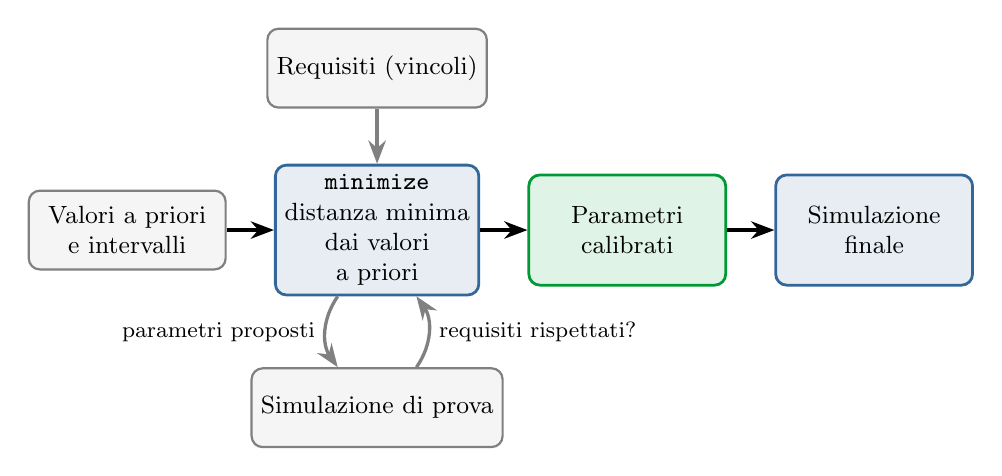
\begin{tikzpicture}[
        block/.style = {
            rectangle, rounded corners = 4pt, draw = ColorP, line width = 1pt, fill = ColorP!12,
            minimum width = 2.5cm, minimum height = 1.4cm, align = center, font = \small
        },
        input/.style = {
            rectangle, rounded corners = 4pt, draw = gray, line width = 0.8pt, fill = gray!8,
            minimum width = 2.5cm, minimum height = 1cm, align = center, font = \small
        },
        flow/.style = {-Stealth, line width = 1.2pt}
    ]
        \node[input] (prior) {Valori a priori\\e intervalli};
        \node[block, right = 0.6cm of prior] (minimize) {\texttt{minimize}\\distanza minima\\dai valori\\a priori};
        \node[block, draw = ColorS, fill = ColorS!12, right = 0.6cm of minimize] (calibrated) {Parametri\\calibrati};
        \node[block, right = 0.6cm of calibrated] (simulation) {Simulazione\\finale};

        \node[input, above = 0.7cm of minimize] (requirements) {Requisiti (vincoli)};
        \node[input, below = 0.9cm of minimize] (trial) {Simulazione di prova};

        \draw[flow] (prior) -- (minimize);
        \draw[flow] (minimize) -- (calibrated);
        \draw[flow] (calibrated) -- (simulation);
        \draw[flow, draw = gray] (requirements) -- (minimize);
        \draw[flow, draw = gray] ([xshift = -0.5cm] minimize.south) to[bend right = 35]
            node[left, font = \footnotesize] {parametri proposti} ([xshift = -0.5cm] trial.north);
        \draw[flow, draw = gray] ([xshift = 0.5cm] trial.north) to[bend right = 35]
            node[right, font = \footnotesize] {requisiti rispettati?} ([xshift = 0.5cm] minimize.south);
    \end{tikzpicture}
    \caption{La procedura di calibrazione dei parametri}\label{fig:calibrazione}
\end{figure}



I parametri calcolati sono riportati nella \autoref{tab:sim-calibrati}. Essi risultano tutti vicini ai valori a priori: la maggior parte cambia di pochi millesimi. \par

I moltiplicatori di abbandono dei sani e dei pregressi restano praticamente invariati. Le correzioni interessano soprattutto i malconci e gli infortunati. Il moltiplicatore di abbandono dei malconci $\beta_M$ passa da $0.050$ a $0.059$ e quello degli infortunati $\beta_I$ da $0.100$ a $0.105$: abbandonano un po' di più, e ciò porta la popolazione finale dall'$87\%$ all'$85\%$ richiesto. Il tasso di recupero parziale $\rho$ passa da $0.050$ a $0.054$: gli infortunati gravi tornano ad allenarsi un po' prima, in media dopo circa $18.7$ sedute anziché $20$, e questo abbassa il picco di infortunati gravi al $10\%$. \par

Con questi parametri, nel momento di massima fatica un atleta sano ha una probabilità di infortunarsi in una singola seduta di circa l'$1.7\%$, un atleta con infortunio pregresso di circa il $3.2\%$ e un malconcio di circa il $6.2\%$.

\begin{table}[ht]
    \centering
    \caption{Parametri del modello: valori a priori e valori calibrati}\label{tab:sim-calibrati}
    \begin{tblr}{
        colspec = {ccc},
    }
        Parametro & Valore a priori & Valore calibrato \\
        $\alpha$ & $0.800$ & $0.800$ \\
        $\pi$ & $0.400$ & $0.397$ \\
        $\rho$ & $0.050$ & $0.054$ \\
        $\beta_S$ & $0.005$ & $0.005$ \\
        $\beta_P$ & $0.010$ & $0.010$ \\
        $\beta_M$ & $0.050$ & $0.059$ \\
        $\beta_I$ & $0.100$ & $0.105$ \\
        $\gamma_S$ & $0.020$ & $0.021$ \\
        $\gamma_P$ & $0.040$ & $0.040$ \\
        $\gamma_M$ & $0.080$ & $0.078$ \\
    \end{tblr}
\end{table}

La \autoref{tab:sim-confronto} confronta i risultati ottenuti con i valori a priori e con i valori calibrati. Le correzioni sono modeste e lo scenario muta poco: il gruppo finale passa da $436$ a $425$ atleti, il picco di infortunati gravi resta intorno ai $52$ atleti e gli infortuni totali passano da circa $417$ a circa $428$. \\
Con infortuni totali non si intendono le singole persone che si sono infortunate, bensì il numero complessivo di infortuni verificatisi. Infatti lo stesso atleta può infortunarsi più di una volta.

\begin{table}[ht]
    \centering
    \caption{Risultati della simulazione con i valori a priori e con i valori calibrati}\label{tab:sim-confronto}
    \begin{tblr}{
        colspec = {lcc},
    }
        & Valori a priori & Valori calibrati \\
        Popolazione massima & $110\%$ & $110\%$ \\
        Popolazione finale & $87\%$ & $85\%$ \\
        Picco di infortunati gravi & $53$ ($10.2\%$) & $52$ ($10\%$) \\
        Picco di malconci & $126$ & $131$ \\
        Massimo di infortunati e malconci & $35\%$ & $36\%$ \\
        Infortuni totali & $417$ & $428$ \\
    \end{tblr}
\end{table}

\subsection{Popolazione totale}

La \autoref{fig:sim-totale} mostra la popolazione totale rispetto a quella iniziale. Si possono distinguere tre fasi. \par

Nella prima fase, nel corso delle prime due settimane, il gruppo cresce grazie ai nuovi ingressi: dopo $10$ sedute è già al $108\%$ di quello iniziale. Nella seconda fase, nella parte centrale del periodo, il gruppo si mantiene stabile intorno al $110\%$: gli ingressi sono terminati e gli abbandoni non sono ancora iniziati. Il massimo, circa $549$ atleti, viene raggiunto intorno alla venticinquesima seduta. \par

Nella terza fase, nell'ultimo terzo del periodo, iniziano gli abbandoni e il gruppo cala. Intorno alla quarantaquattresima seduta torna sotto il valore iniziale, alla quarantacinquesima è al $97\%$ e alla fine arriva a $425$ atleti, cioè l'$85\%$ di quello iniziale, come richiesto. \par

\begin{figure}[ht]
    \centering
    \includegraphics[width = \textwidth]{simulazione/popolazione_totale.pdf}
    \caption{Popolazione totale rispetto a quella iniziale}\label{fig:sim-totale}
\end{figure}

Complessivamente abbandonano circa $124$ atleti: soltanto $12$ sani e $4$ pregressi, contro $44$ infortunati e $64$ malconci. Gli infortunati e i malconci, che all'inizio non esistevano, sono dunque responsabili dell'$87\%$ degli abbandoni. Gli infortuni costituiscono la causa principale della riduzione del gruppo: ridurre gli infortuni significherebbe anche mantenere unito il gruppo.

\subsection{Le quattro popolazioni}

La \autoref{fig:sim-popolazioni} mostra le quattro popolazioni e la \autoref{tab:sim-popolazioni} ne riporta i valori ogni dieci sedute.

\begin{figure}[ht]
    \centering
    \includegraphics[width = \textwidth]{simulazione/popolazioni.pdf}
    \caption{Le quattro popolazioni con i parametri calibrati}\label{fig:sim-popolazioni}
\end{figure}

\begin{table}[ht]
    \centering
    \caption{Le quattro popolazioni ogni dieci sedute}\label{tab:sim-popolazioni}
    \begin{tblr}{
        colspec = {cccccc},
    }
        Seduta & $S$ & $P$ & $I$ & $M$ & Infortunati e malconci \\
        $0$ & $400$ & $100$ & $0$ & $0$ & $0\%$ \\
        $10$ & $399$ & $93$ & $17$ & $32$ & $9\%$ \\
        $20$ & $370$ & $79$ & $31$ & $68$ & $18\%$ \\
        $30$ & $333$ & $65$ & $44$ & $106$ & $27\%$ \\
        $40$ & $293$ & $51$ & $52$ & $131$ & $35\%$ \\
        $50$ & $243$ & $36$ & $38$ & $108$ & $34\%$ \\
    \end{tblr}
\end{table}

Nelle prime sedute i sani rimangono quasi costanti, poiché i nuovi ingressi compensano gli infortuni; successivamente, sia i sani sia i pregressi diminuiscono per tutto il periodo. La diminuzione è dovuta soprattutto agli infortuni, che li spostano tra i malconci o tra gli infortunati, mentre gli abbandoni incidono poco. I pregressi diminuiscono più rapidamente dei sani in proporzione, perché presentano un rischio di infortunio più elevato: alla fine ne restano $36$ su $100$, mentre i sani sono $243$ su $400$. \par

Gli infortunati e i malconci partono da zero e crescono per gran parte del periodo. Raggiungono il massimo intorno alla quarantesima seduta, con circa $52$ infortunati e $131$ malconci, per poi diminuire a causa degli abbandoni. I malconci superano i pregressi già intorno alla ventitreesima seduta, ma infortunati e malconci insieme restano sempre meno numerosi di sani e pregressi insieme. \par

I malconci sono sempre più numerosi degli infortunati gravi, per due ragioni. La prima è che la maggior parte degli infortuni è lieve e conduce l'atleta direttamente in $M$. La seconda è che anche gli infortunati gravi, quando guariscono parzialmente, passano in $M$. I malconci, a loro volta, presentano il rischio di infortunio più alto e possono infortunarsi gravemente, tornando in $I$. \par

Al termine del periodo restano $243$ sani, $36$ pregressi, $38$ infortunati e $108$ malconci: circa un terzo degli atleti rimasti è infortunato o malconcio.

\subsection{Infortunati}

La \autoref{fig:sim-frazioni} mostra la frazione di infortunati gravi e quella di infortunati e malconci insieme. Entrambe crescono in modo regolare per gran parte del periodo. Gli infortunati gravi raggiungono il $10\%$ del gruppo intorno alla quarantaduesima seduta, senza mai superarlo. Infortunati e malconci insieme arrivano al massimo al $36\%$ del gruppo, rimanendo quindi ben al di sotto del limite del $50\%$. Nelle ultime sedute entrambe le frazioni diminuiscono leggermente, non perché vi siano meno infortuni, ma perché molti infortunati e malconci abbandonano. \par

\begin{figure}[ht]
    \centering
    \includegraphics[width = \textwidth]{simulazione/frazione_infortunati.pdf}
    \caption{Frazione di infortunati gravi e di infortunati e malconci}\label{fig:sim-frazioni}
\end{figure}

Complessivamente si verificano circa $428$ infortuni, di cui $170$ gravi e $258$ lievi. In media si verificano circa $9$ infortuni per seduta, ma il numero cresce nel tempo insieme alla fatica: sono circa $4$ nella prima seduta e arrivano a circa $13$ intorno alla quarantatreesima. Nella seconda metà del periodo si verificano circa $270$ infortuni, contro i $158$ della prima metà. \par

Gli infortuni si distribuiscono tra le popolazioni nel modo seguente: circa $184$ riguardano i sani, $70$ i pregressi e $174$ i malconci. I malconci, pur essendo molto meno numerosi dei sani, producono il $41\%$ degli infortuni, quasi quanto i sani, perché costituiscono la popolazione più a rischio. La \autoref{fig:sim-infortuni-popolazione} mostra questa ripartizione. \par

\begin{figure}[ht]
    \centering
    \includegraphics[width = \textwidth]{simulazione/infortuni_per_popolazione.pdf}
    \caption{Infortuni per popolazione di provenienza}\label{fig:sim-infortuni-popolazione}
\end{figure}


Una parte degli atleti si infortuna più di una volta, ad esempio prima in modo lieve, diventando malconci, e poi in modo grave. Rapportando gli infortuni al numero di presenze sul tatami si ottengono circa $17$ infortuni ogni $1000$ presenze, un valore elevato, coerente con uno scenario privo di prevenzione.

\section{Analisi di sensibilità}\label{sec:sensibilita}

I parametri del modello non sono stimati a partire da dati reali, ma scelti con la calibrazione per plausibilità. È quindi importante capire quanto i risultati dipendano dai valori scelti. Per farlo abbiamo ripetuto la simulazione variando un parametro alla volta del $20\%$ in più e in meno rispetto al suo valore, lasciando invariati tutti gli altri. Questo approccio, detto ``one-at-a-time'', è il metodo più semplice di analisi di sensibilità~\cite{pianosi2016}. Abbiamo considerato quattordici parametri: i moltiplicatori di rischio e di abbandono dei malconci e degli infortunati, la probabilità $\pi$, il tasso di recupero parziale $\rho$, i parametri della funzione di infortunio, la capienza del tatami, la velocità di decadimento del recupero e l'ampiezza degli ingressi. \par

La \autoref{fig:sim-sensibilita} mostra la variazione degli infortuni totali, con i parametri ordinati dal più influente al meno influente, e la \autoref{tab:sim-sensibilita} riporta i valori.

\begin{figure}[ht]
    \centering
    \includegraphics[width = \textwidth]{simulazione/sensibilita.pdf}
    \caption{Variazione degli infortuni totali al variare di ciascun parametro del $20\%$}\label{fig:sim-sensibilita}
\end{figure}

\begin{table}[ht]
    \centering
    \caption{Infortuni totali e riduzione con la prevenzione al variare di ciascun parametro del $20\%$}\label{tab:sim-sensibilita}
    \begin{tblr}{
        colspec = {X[c, m] X[c, m] X[c, m] X[c, m] X[c, m]},
        width = \textwidth,
        hline{2} = {0pt},
        hline{2} = {2-3}{leftpos = -1, rightpos = -1, endpos, 0.05em},
        hline{2} = {4-5}{leftpos = -1, rightpos = -1, endpos, 0.05em},
        hline{3} = {0.05em},
    }
        \SetCell[r=2]{c} Parametro & \SetCell[c=2]{c} Infortuni totali & & \SetCell[c=2]{c} Riduzione con prevenzione & \\
        & $-20\%$ & $+20\%$ & $-20\%$ & $+20\%$ \\
        $\gamma_S$ & $377$ & $474$ & $31.2\%$ & $30.4\%$ \\
        $b$ & $471$ & $385$ & $31.0\%$ & $30.7\%$ \\
        $\sigma_r$ & $391$ & $469$ & $30.7\%$ & $31.0\%$ \\
        $\gamma_M$ & $397$ & $457$ & $30.0\%$ & $31.5\%$ \\
        $\omega_f$ & $403$ & $452$ & $31.0\%$ & $30.7\%$ \\
        $\gamma_P$ & $411$ & $442$ & $31.2\%$ & $30.5\%$ \\
        $\omega_p$ & $413$ & $443$ & $31.0\%$ & $30.8\%$ \\
        $\pi$ & $442$ & $415$ & $31.4\%$ & $30.3\%$ \\
        $\omega_\mu$ & $421$ & $435$ & $30.9\%$ & $30.8\%$ \\
        $\rho$ & $421$ & $434$ & $30.5\%$ & $31.1\%$ \\
        $A_{\max}$ & $435$ & $424$ & $30.9\%$ & $30.9\%$ \\
        $\omega_d$ & $423$ & $433$ & $30.9\%$ & $30.9\%$ \\
        $\beta_M$ & $431$ & $425$ & $30.9\%$ & $30.8\%$ \\
        $\beta_I$ & $428$ & $428$ & $30.9\%$ & $30.8\%$ \\
    \end{tblr}
\end{table}

Nessuna variazione modifica gli infortuni totali di più del $12\%$: con parametri variati del $20\%$, gli infortuni restano compresi tra circa $377$ e $474$, contro i $428$ dello scenario di riferimento. Il modello, quindi, non amplifica le incertezze sui parametri. \par

I parametri più influenti sono quelli del rischio e del recupero. Il primo è il moltiplicatore di rischio dei sani $\gamma_S$, perché i sani sono la popolazione più numerosa. Seguono la soglia $b$, che con un valore più alto riduce il rischio di base, la velocità di decadimento del recupero $\sigma_r$, il moltiplicatore di rischio dei malconci $\gamma_M$ e il peso della fatica fisica $\omega_f$. I parametri degli abbandoni, $\beta_M$ e $\beta_I$, la capienza del tatami $A_{\max}$ e il peso della densità $\omega_d$ incidono invece per meno del $2\%$: gli abbandoni si concentrano nelle ultime sedute, quando la maggior parte degli infortuni è già avvenuta, e la densità varia poco nel corso del periodo. \par

Un risultato meno intuitivo riguarda la probabilità $\pi$ che un infortunio sia grave: aumentandola, gli infortuni totali diminuiscono. Con più infortuni gravi, infatti, più atleti si fermano in $I$, dove non sono esposti al rischio, e meno atleti diventano malconci, che sono la popolazione più a rischio. Il numero di infortuni gravi aumenta, ma il numero complessivo diminuisce. \par

Anche la popolazione finale varia poco: in tutti i casi resta compresa tra l'$83\%$ e l'$87\%$ di quella iniziale. \par

Infine, l'analisi riguarda anche la prevenzione che introdurremo nel capitolo successivo. La riduzione degli infortuni ottenuta con la prevenzione è praticamente insensibile ai parametri: in tutti i casi resta compresa tra il $30.0\%$ e il $31.5\%$.

\section{Considerazioni finali}

Lo scenario ottenuto descrive un periodo di allenamento intenso senza prevenzione: si verificano circa $428$ infortuni, il gruppo perde il $15\%$ degli atleti e alla fine circa un terzo degli atleti rimasti è infortunato o malconcio. Al tempo stesso, lo scenario rispetta tutti i requisiti: la popolazione non cresce più del $10\%$, alla fine è l'$85\%$ di quella iniziale, gli infortunati gravi non superano il $10\%$ e gli infortunati e i malconci non superano la metà del gruppo. \par

Dai risultati emergono tre aspetti sui quali il controllo potrà intervenire:
\begin{itemize}
    \item il rischio di infortunio cresce con la fatica, e difatti gli infortuni sono più numerosi nella seconda metà del periodo: ridurre la fatica, ad esempio modificando l'alternanza tra sedute intense e sedute di recupero, riduce gli infortuni;
    \item i malconci sono la popolazione più a rischio e producono circa il $41\%$ degli infortuni: una strategia di prevenzione mirata a loro, ad esempio riducendone il carico, può avere un effetto rilevante;
    \item gli infortunati e i malconci sono la causa principale degli abbandoni: ridurre gli infortuni aiuta anche a mantenere unito il gruppo.
\end{itemize}

I parametri scelti non sono stimati a partire da dati reali, bensì dai requisiti che abbiamo fissato e dai valori a priori. Con requisiti o valori a priori differenti si otterrebbe uno scenario diverso. Lo scenario va dunque inteso come un caso di riferimento, utile per confrontare strategie diverse, e non come una previsione di ciò che accade in una palestra reale. L'analisi di sensibilità mostra comunque che variazioni moderate dei parametri non cambiano la forma della dinamica né le conclusioni qualitative. Disporre anche di pochi dati reali, come il numero di iscritti, di abbandoni e di infortuni in una stagione, permetterebbe di scegliere i requisiti in modo più oggettivo.

    \chapter{Modello con controllo}

Nel capitolo precedente abbiamo simulato il modello senza alcuna forma di prevenzione e abbiamo ottenuto uno scenario sfavorevole: in un periodo di cinquanta sedute si verificano circa $428$ infortuni, il gruppo perde il $15\%$ degli atleti, quasi tutti infortunati o malconci, e alla fine circa un terzo degli atleti rimasti è infortunato o malconcio. Questo scenario descrive che cosa succede quando l'allenatore si limita a proporre il programma di allenamento, senza intervenire per ridurre il rischio. \par

Nella pratica, però, l'allenatore ha a disposizione diversi strumenti per prevenire gli infortuni. Può dedicare più tempo al riscaldamento e alla mobilità articolare, inserire esercizi di rinforzo muscolare e di propriocezione, controllare con più attenzione le coppie sul tatami, ad esempio evitando che atleti di peso o livello molto diversi lavorino insieme, oppure ridurre il numero di atleti che combattono contemporaneamente. Tutte queste azioni hanno lo stesso effetto: rendono meno probabile che un atleta si infortuni durante la seduta. \par

In questo capitolo introduciamo nel modello un termine di controllo, indicato con $u(t)$, che rappresenta l'efficacia della prevenzione nella seduta $t$. Il controllo è la variabile su cui l'allenatore può agire: a differenza dei parametri del modello, che descrivono le caratteristiche del gruppo, il controllo descrive una scelta, e può cambiare da una seduta all'altra. \par

La prevenzione, però, non è gratuita. Ogni minuto dedicato al riscaldamento o agli esercizi di rinforzo è un minuto sottratto alla tecnica e al randori, e un controllo più attento delle coppie richiede tempo e attenzione da parte dell'allenatore. Non è quindi realistico pensare di applicare la massima prevenzione in ogni seduta. La domanda a cui vogliamo rispondere è allora la seguente: se l'allenatore dedica alla prevenzione un impegno proporzionato alla fatica di ciascuna seduta, di quanto si riducono gli infortuni e gli abbandoni? \par

Per rispondere a questa domanda manteniamo fisso tutto il resto. I parametri del modello e delle funzioni sono quelli calibrati nel capitolo precedente, e il carico di allenamento è lo stesso carico periodico. In questo modo le differenze tra le simulazioni dipendono soltanto dal controllo, e lo scenario senza prevenzione diventa il termine di confronto per misurare l'efficacia di ciascuna strategia.

\section{Il modello con il controllo}

Il controllo $u(t)$ rappresenta l'efficacia della prevenzione nella seduta $t$, ed è un numero compreso tra $0$ e $1$:
\[
    u(t) \in [0, 1] \quad \text{con } t = 0, 1, \dots, T - 1
\]
Il valore $u(t) = 0$ corrisponde all'assenza di prevenzione: la seduta si svolge come nel capitolo precedente. Il valore $u(t) = 1$ corrisponde a una prevenzione perfetta, che elimini completamente il rischio di infortunio in quella seduta. I valori intermedi rappresentano una prevenzione parziale: ad esempio, $u(t) = 0.3$ significa che le misure adottate riducono del $30\%$ la probabilità di infortunio di ogni atleta. \par

La prevenzione perfetta è naturalmente un caso limite, che non si può raggiungere nella pratica: anche con tutte le precauzioni possibili, in uno sport di contatto come il judo resta sempre un rischio residuo. Il valore $u(t) = 1$ serve soprattutto come riferimento, mentre le strategie realistiche useranno valori più bassi. \par

Il controllo può cambiare da una seduta all'altra. L'allenatore può decidere, ad esempio, di concentrare la prevenzione nei giorni di randori, quando il carico è più alto, oppure nella seconda parte del periodo, quando la fatica accumulata è maggiore. Per questo motivo il controllo è una funzione del tempo e non un singolo numero.

\subsection{Le equazioni}

Il controllo agisce soltanto sul rischio di infortunio. La probabilità che un atleta di una popolazione si infortuni nella seduta $t$, che senza prevenzione è $\tilde\lambda_\cdot(t)$, diventa
\[
    (1 - u(t)) \tilde\lambda_\cdot(t)
\]
cioè viene ridotta della frazione $u(t)$. \par

Usando le stesse abbreviazioni definite in \autoref{sec:model-complete}:
\begin{gather*}
    \tilde\mu(t) = \mu\left(\frac{t}{T}\right) \\
    \tilde\nu_\cdot(t) = \nu\left(\frac{t}{T}, \beta_\cdot\right) \\
    \tilde\lambda_\cdot(t) = \lambda\left(\bar{F}_f(t), \bar{F}_p(t), \frac{S(t) + P(t) + M(t)}{A_{\max}}, \gamma_\cdot\right)
\end{gather*}
il modello con il controllo si può scrivere come:
\begin{equation*}
    \begin{aligned}
        S(t+1) &= S(t)
            + \alpha \tilde\mu(t)
            - \tilde\nu_S(t) S(t)
            - (1 - u(t)) \tilde\lambda_S(t) S(t) \\[10pt]
        P(t+1) &= P(t)
            + (1 - \alpha) \tilde\mu(t)
            - \tilde\nu_P(t) P(t)
            - (1 - u(t)) \tilde\lambda_P(t) P(t) \\[10pt]
        I(t+1) &= I(t)
            - \rho I(t)
            - \tilde\nu_I(t) I(t) \\
            &+ \pi (1 - u(t)) \left( \tilde\lambda_S(t) S(t)
            + \tilde\lambda_P(t) P(t)
            + \tilde\lambda_M(t) M(t) \right) \\[10pt]
        M(t+1) &= M(t)
            + \rho I(t)
            - \tilde\nu_M(t) M(t) \\
            &+ (1 - \pi) (1 - u(t)) \tilde\lambda_S(t) S(t)
            + (1 - \pi) (1 - u(t)) \tilde\lambda_P(t) P(t) \\
            &- \pi (1 - u(t)) \tilde\lambda_M(t) M(t) \\[10pt]
        \bar{F}_f(t+1) &= \bar{F}_f(t)
            + c_f(t)
            - r(t) \bar{F}_f(t) \\[10pt]
        \bar{F}_p(t+1) &= \bar{F}_p(t)
            + c_p(t)
            - r(t) \bar{F}_p(t)
    \end{aligned}
\end{equation*}

Rispetto al modello senza controllo, l'unica differenza è il fattore $(1 - u(t))$ davanti a tutti i termini di infortunio. Tutti gli altri flussi restano invariati: gli ingressi, gli abbandoni, il recupero parziale da $I$ a $M$ e l'accumulo della fatica non dipendono dalla prevenzione. \par

Questa scelta riflette il tipo di prevenzione che stiamo considerando. Il riscaldamento, gli esercizi di rinforzo e il controllo delle coppie riducono la probabilità di infortunarsi, ma non cambiano il carico della seduta, e quindi non cambiano la fatica accumulata dagli atleti. Allo stesso modo, la prevenzione non aiuta gli atleti già infortunati a guarire più in fretta e non influisce direttamente sulla loro decisione di abbandonare. \par

Va notato, però, che il controllo ha anche effetti indiretti. Riducendo gli infortuni, la prevenzione mantiene più atleti nelle popolazioni $S$ e $P$, che abbandonano meno degli infortunati e dei malconci. Inoltre mantiene più atleti sul tatami, e quindi modifica la densità e, di conseguenza, il rischio delle sedute successive. Per questo motivo l'effetto complessivo di una strategia di prevenzione non si può calcolare semplicemente moltiplicando il numero di infortuni per $(1 - u)$, ma richiede di simulare il modello. \par

Il diagramma dei flussi è lo stesso del modello senza controllo, con l'unica differenza che le frecce che rappresentano gli infortuni, cioè quelle da $S$ e da $P$ verso $I$ e $M$ e quella da $M$ verso $I$, sono moltiplicate per $(1 - u(t))$. Quando $u(t)$ è vicino a $1$ queste frecce diventano molto sottili: gli atleti restano nelle popolazioni di partenza e si allenano senza infortunarsi. Quando $u(t)$ è vicino a $0$ il diagramma coincide con quello del capitolo sul modello.

\subsection{Proprietà del modello con il controllo}

L'introduzione del controllo non modifica le proprietà principali del modello, che continuano a valere per qualsiasi scelta di $u(t)$ compresa tra $0$ e $1$.

\paragraph{Il modello senza controllo è un caso particolare}
Se $u(t) = 0$ per ogni seduta, il fattore $(1 - u(t))$ vale $1$ e le equazioni coincidono con quelle del modello senza controllo. Lo scenario del capitolo precedente è quindi il caso particolare in cui l'allenatore non fa alcuna prevenzione. Questa proprietà è stata verificata anche nelle simulazioni: con il controllo nullo si ottengono esattamente gli stessi risultati del capitolo precedente.

\paragraph{Le popolazioni restano non negative}
Poiché $u(t) \geq 0$, il rischio effettivo $(1 - u(t)) \tilde\lambda_\cdot(t)$ è sempre minore o uguale al rischio senza controllo $\tilde\lambda_\cdot(t)$. Le uscite da ciascuna popolazione possono quindi solo diminuire, e i vincoli di integrità del modello senza controllo continuano a valere. In particolare, se le popolazioni restano non negative senza prevenzione, restano non negative anche con qualsiasi strategia di prevenzione.

\paragraph{La popolazione totale si conserva}
Il controllo moltiplica tutti i termini di infortunio per lo stesso fattore, sia quando un atleta esce da una popolazione sia quando entra in un'altra. Gli infortuni continuano quindi a spostare gli atleti tra le popolazioni senza crearne né eliminarne, e la popolazione totale continua a cambiare soltanto per effetto degli ingressi e degli abbandoni:
\[
    N(t+1) = N(t) + \tilde\mu(t) - \tilde\nu_S(t) S(t) - \tilde\nu_P(t) P(t) - \tilde\nu_I(t) I(t) - \tilde\nu_M(t) M(t).
\]
Il controllo, però, cambia la composizione del gruppo, e quindi cambia indirettamente anche gli abbandoni: con più atleti sani e meno infortunati, gli abbandoni complessivi diminuiscono.

\paragraph{La fatica non dipende dal controllo}
Le equazioni della fatica non contengono $u(t)$. Con lo stesso carico di allenamento, la fatica media del gruppo è la stessa per qualsiasi strategia di prevenzione. La prevenzione non rende gli atleti meno stanchi, ma riduce le conseguenze della stanchezza sul rischio di infortunio. Il rischio relativo $\frac{\tilde\lambda_\cdot}{\gamma_\cdot}$ cambia invece leggermente da una strategia all'altra, ma solo attraverso la densità sul tatami: con la prevenzione restano più atleti ad allenarsi, e il tatami è un po' più affollato.

\subsection{La strategia di prevenzione}

Se la prevenzione non avesse alcun costo, la strategia migliore sarebbe banale: applicare la massima prevenzione possibile in ogni seduta. Come abbiamo detto, però, la prevenzione richiede tempo e attenzione, e il tempo dedicato alla prevenzione viene sottratto all'allenamento vero e proprio. È quindi ragionevole dedicarle più spazio nelle sedute più impegnative e meno spazio in quelle leggere. \par

Per questo motivo scegliamo una prevenzione proporzionale al carico della seduta:
\[
    u(t) = u_{\text{base}} \cdot c(t),
\]
dove $u_{\text{base}}$ è la prevenzione applicata nel giorno di randori. Con il carico periodico del capitolo precedente, questa scelta dà:
\begin{itemize}
    \item nel giorno di randori, quando il carico è massimo, la prevenzione vale $u_{\text{base}}$;
    \item nel giorno di tecnica, quando il carico è la metà, anche la prevenzione è la metà, cioè $\frac{u_{\text{base}}}{2}$;
    \item nel giorno di riposo, quando il carico è nullo, non si fa prevenzione.
\end{itemize}
Questa strategia corrisponde a un comportamento naturale per un allenatore: riscaldamento più lungo, esercizi di rinforzo e un controllo più attento delle coppie nei giorni di randori, una prevenzione più leggera nei giorni di tecnica e nessuna attività particolare nei giorni di riposo. \par

Nelle simulazioni usiamo $u_{\text{base}} = 0.6$: nel giorno di randori la prevenzione riduce del $60\%$ il rischio di infortunio, nel giorno di tecnica del $30\%$. In media, su tutto il periodo, la prevenzione vale circa $0.3$ per seduta.

    \chapter{Conclusioni}

Questa tesi ha avuto come obiettivo la costruzione di un modello matematico in grado di descrivere l'evoluzione, seduta dopo seduta, di un gruppo di judoka nel corso di un periodo di allenamento, allo scopo di analizzare gli infortuni e l'incidenza della prevenzione. \par

Gli atleti sono suddivisi dal modello in quattro popolazioni: i sani, coloro che hanno subito infortuni pregressi, gli infortunati gravi, impossibilitati ad allenarsi, e i malconci, che continuano ad allenarsi nonostante un infortunio lieve o una guarigione incompleta. A queste popolazioni si affiancano due variabili che rappresentano la fatica media del gruppo, nella componente fisica e in quella psicologica. Cinque funzioni governano il passaggio da una popolazione all'altra: esse descrivono l'arrivo di nuovi atleti, gli abbandoni, gli infortuni, il carico di allenamento e il recupero. Tra queste, la funzione di infortunio riveste il ruolo principale, poiché mette in relazione il rischio con la fatica del gruppo e con la densità di atleti presenti sul tatami. \par

Per ogni funzione abbiamo adottato una forma analitica semplice, dotata di parametri interpretabili, e ne abbiamo esaminato le proprietà. In mancanza di dati reali, abbiamo proceduto a una calibrazione per plausibilità: dopo aver stabilito alcuni requisiti che la dinamica del gruppo deve soddisfare, abbiamo individuato, tramite la libreria SciPy, i parametri più prossimi a una stima iniziale che li rispettano. Ne è derivato uno scenario di riferimento che rappresenta un periodo di allenamento intenso privo di prevenzione. \par

Abbiamo infine inserito nel modello un controllo, che esprime l'efficacia della prevenzione attuata dall'allenatore e riduce il rischio di infortunio per tutte le popolazioni. Abbiamo quindi simulato una strategia di prevenzione commisurata al carico, più incisiva nei giorni di randori, ridotta della metà nei giorni di tecnica e del tutto assente nelle sedute leggere, confrontandola con lo scenario privo di prevenzione.

\section{Risultati principali}

Nello scenario senza prevenzione, nell'arco di cinquanta sedute si registrano circa $428$ infortuni e il gruppo perde il $15\%$ dei propri atleti. La quasi totalità degli abbandoni, circa l'$87\%$, riguarda atleti infortunati o malconci, e al termine del periodo circa un terzo degli atleti rimasti non si trova in condizioni ottimali. \par

Le simulazioni hanno messo in luce tre aspetti fondamentali.
\begin{itemize}
    \item \textbf{La fatica accresce il rischio.} Il rischio di infortunio aumenta con la fatica accumulata, e difatti gli infortuni risultano più frequenti nella seconda metà del periodo. Il nesso tra carico di allenamento, fatica e rischio di infortunio costituisce un tema centrale della medicina dello sport~\cite{soligard2016}. La scelta della funzione di recupero si è dimostrata determinante: qualora il recupero cali troppo rapidamente, la fatica cresce senza limite, il rischio raggiunge il valore massimo e il carico di allenamento perde ogni effetto sugli infortuni.
    \item \textbf{I malconci costituiscono la popolazione più critica.} Benché siano meno numerosi dei sani, essi producono circa il $41\%$ degli infortuni, in quanto popolazione più esposta al rischio. Essi alimentano inoltre un ciclo nel quale gli infortuni lievi conducono a nuovi infortuni gravi.
    \item \textbf{Gli infortuni determinano gli abbandoni.} Gli infortunati e i malconci abbandonano con molta maggiore facilità rispetto agli atleti sani. Ridurre gli infortuni equivale dunque anche a mantenere unito il gruppo.
\end{itemize}

La prevenzione proporzionale al carico, con una prevenzione media di circa $0.3$ per seduta, determina una riduzione degli infortuni del $31\%$, da circa $428$ a circa $296$, e degli abbandoni del $18\%$, da circa $124$ a circa $102$. L'effetto risulta particolarmente marcato sui malconci, i cui infortuni calano quasi della metà, poiché la prevenzione impedisce che molti atleti diventino malconci. Infine, l'effetto della prevenzione cresce in modo regolare con l'intensità: anche una prevenzione leggera produce un beneficio apprezzabile. La \autoref{fig:riepilogo} riassume il confronto tra i due scenari.

\begin{figure}[ht]
    \centering
    \includegraphics[width = \textwidth]{conclusioni/riepilogo.pdf}
    \caption{Infortuni e abbandoni totali, con e senza prevenzione}\label{fig:riepilogo}
\end{figure}


\section{Limiti del modello}

Il modello costituisce una semplificazione della realtà, e talune scelte compiute per mantenerlo semplice ne circoscrivono la validità. È opportuno esplicitarle, sia per interpretare correttamente i risultati sia per individuare possibili miglioramenti.

\paragraph{Assenza di dati reali}

Il limite principale risiede nel fatto che i parametri non sono stati stimati a partire da dati reali. La calibrazione per plausibilità assicura che la dinamica del gruppo sia ragionevole, ma il risultato dipende da due scelte soggettive: i valori iniziali dei parametri e le soglie dei requisiti, quali il calo della popolazione o il picco di infortunati gravi. Scelte differenti condurrebbero a uno scenario diverso. \par

Per tale ragione i numeri ottenuti, come i circa $428$ infortuni o la riduzione del $31\%$ attribuibile alla prevenzione, non devono essere interpretati come previsioni di quanto accade in una palestra reale. Essi assumono valore soprattutto nel confronto tra scenari differenti: risulta ad esempio più affidabile l'affermazione secondo cui la prevenzione riduce gli infortuni dei malconci più di quelli dei sani, rispetto al valore esatto della riduzione. Inoltre, combinazioni diverse di parametri possono generare traiettorie simili, e in assenza di dati non è possibile stabilire quale sia quella corretta. Gli studi sugli infortuni nel judo reperibili in letteratura descrivono soprattutto la frequenza e la tipologia degli infortuni \cite{pocecco2013}, ma non seguono l'evoluzione di un gruppo di atleti seduta dopo seduta, che è quanto servirebbe per stimare i parametri del modello.

\paragraph{La fatica è identica per tutti}

Il modello impiega un'unica fatica media per l'intero gruppo, scelta giustificata dalle ipotesi di omogeneità, mescolamento e simmetria. Nella realtà, tuttavia, la fatica varia da atleta ad atleta: un malconcio è verosimilmente più affaticato di un sano, e un atleta appena rientrato da un infortunio lo è meno di uno che si è allenato per l'intero periodo. Il modello non è in grado di rappresentare tali differenze, né la possibilità che un allenatore assegni carichi differenti ad atleti differenti. Inoltre, nelle simulazioni il carico fisico e quello psicologico coincidono, per cui la distinzione tra le due componenti della fatica, pur presente nel modello, non è stata sfruttata.

\paragraph{Il recupero e l'orizzonte temporale}

La funzione di recupero adottata tende a zero con il trascorrere del tempo. Su un orizzonte di cinquanta sedute ciò non rappresenta un problema, poiché il recupero diminuisce lentamente e al termine del periodo vale ancora circa $0.15$. Su orizzonti più estesi, invece, la fatica crescerebbe senza limite e il rischio raggiungerebbe il valore massimo, con gli stessi problemi osservati per il recupero che decade rapidamente. Per orizzonti lunghi sarebbe pertanto necessario introdurre un valore minimo del recupero.

\paragraph{Ingressi e abbandoni}

Ingressi e abbandoni dipendono unicamente dal tempo, e la popolazione a cui si applicano interviene soltanto attraverso un moltiplicatore. Nella realtà, al contrario, la decisione di abbandonare può dipendere dalla fatica, dalla durata di un infortunio o dal clima del gruppo, mentre gli ingressi possono dipendere dalla dimensione del gruppo o dal periodo dell'anno. Il modello coglie tali differenze solo indirettamente, mediante i diversi moltiplicatori di abbandono delle quattro popolazioni.

\paragraph{Il controllo}

Il controllo è stato modellato nella forma più semplice possibile: riduce il rischio di infortunio di una frazione determinata, identica per tutte le popolazioni. Tale scelta trascura diversi aspetti:
\begin{itemize}
    \item la prevenzione non comporta alcun costo per l'allenamento: il tempo dedicato al riscaldamento o al rinforzo non riduce il carico né il beneficio della seduta;
    \item la prevenzione non modifica la gravità degli infortuni né la velocità di guarigione, sebbene nella realtà alcune misure, come la fisioterapia, potrebbero incidere su di esse;
    \item la prevenzione è identica per tutte le popolazioni, mentre un allenatore potrebbe riservare maggiore attenzione proprio ai malconci, che risultano i più a rischio;
    \item la strategia di prevenzione è stata scelta a priori e non ottimizzata: non è noto se esista una strategia migliore a parità di prevenzione complessiva.
\end{itemize}

\paragraph{Un modello deterministico}

Il modello è infine deterministico e tratta le popolazioni come numeri reali. Gli infortuni, tuttavia, sono eventi casuali: due periodi di allenamento identici possono presentare un numero di infortuni molto differente. Il modello descrive soltanto l'andamento medio, ed è tanto più affidabile quanto più numeroso è il gruppo. Per gruppi piccoli, come quelli di molte palestre, le fluttuazioni casuali possono assumere rilevanza pari a quella dell'andamento medio.

\section{Sviluppi futuri}

I limiti discussi indicano alcune direzioni naturali per lo sviluppo di questo lavoro.
\begin{itemize}
    \item \textbf{Raccogliere dati reali.} Anche pochi dati, quali il numero di iscritti, di abbandoni e di infortuni in una stagione in una singola palestra, consentirebbero di stimare i parametri anziché sceglierli, e di verificare se il modello descriva correttamente un gruppo reale.
    \item \textbf{Ricercare la strategia ottima.} Anziché scegliere la strategia a priori, si potrebbe individuare quella che riduce maggiormente gli infortuni a parità di prevenzione complessiva, oppure quella che raggiunge un determinato obiettivo con il minimo sforzo, avvalendosi ad esempio delle tecniche del controllo ottimo o dell'apprendimento per rinforzo.
    \item \textbf{Prevenzione mirata.} Consentire una prevenzione differenziata per ciascuna popolazione permetterebbe di studiare strategie rivolte in particolare ai malconci, che i risultati indicano come la popolazione più critica.
    \item \textbf{Il carico come controllo.} Oltre alla prevenzione, anche il carico di allenamento costituisce una scelta dell'allenatore. Considerarlo come seconda variabile di controllo permetterebbe di ricercare un equilibrio tra un allenamento efficace e un numero contenuto di infortuni.
    \item \textbf{Un modello stocastico.} L'introduzione della casualità degli infortuni permetterebbe di descrivere anche gruppi piccoli e di stimare non solo il numero medio di infortuni, ma anche la sua variabilità da un periodo all'altro.
\end{itemize}

In conclusione, il modello proposto è semplice, ma consente già di comprendere alcuni meccanismi rilevanti, quali il legame tra fatica e rischio, il ruolo dei malconci e il nesso tra infortuni e abbandoni, e di confrontare quantitativamente strategie di prevenzione differenti. Con l'aggiunta di dati reali e di alcune delle estensioni proposte, esso potrebbe divenire uno strumento utile per supportare gli allenatori nella progettazione di allenamenti più sicuri.
\end{document}
